% Options for packages loaded elsewhere
\PassOptionsToPackage{unicode}{hyperref}
\PassOptionsToPackage{hyphens}{url}
\PassOptionsToPackage{dvipsnames,svgnames,x11names}{xcolor}
%
\documentclass[
  11pt,
  a4paper,
  DIV=11,
  numbers=noendperiod]{scrartcl}

\usepackage{amsmath,amssymb}
\usepackage{iftex}
\ifPDFTeX
  \usepackage[T1]{fontenc}
  \usepackage[utf8]{inputenc}
  \usepackage{textcomp} % provide euro and other symbols
\else % if luatex or xetex
  \usepackage{unicode-math}
  \defaultfontfeatures{Scale=MatchLowercase}
  \defaultfontfeatures[\rmfamily]{Ligatures=TeX,Scale=1}
\fi
\usepackage{lmodern}
\ifPDFTeX\else  
    % xetex/luatex font selection
\fi
% Use upquote if available, for straight quotes in verbatim environments
\IfFileExists{upquote.sty}{\usepackage{upquote}}{}
\IfFileExists{microtype.sty}{% use microtype if available
  \usepackage[]{microtype}
  \UseMicrotypeSet[protrusion]{basicmath} % disable protrusion for tt fonts
}{}
\makeatletter
\@ifundefined{KOMAClassName}{% if non-KOMA class
  \IfFileExists{parskip.sty}{%
    \usepackage{parskip}
  }{% else
    \setlength{\parindent}{0pt}
    \setlength{\parskip}{6pt plus 2pt minus 1pt}}
}{% if KOMA class
  \KOMAoptions{parskip=half}}
\makeatother
\usepackage{xcolor}
\usepackage[lmargin=2cm,rmargin=2cm,tmargin=2cm,bmargin=2cm]{geometry}
\ifLuaTeX
  \usepackage{luacolor}
  \usepackage[soul]{lua-ul}
\else
  \usepackage{soul}
  
\fi
\setlength{\emergencystretch}{3em} % prevent overfull lines
\setcounter{secnumdepth}{-\maxdimen} % remove section numbering
% Make \paragraph and \subparagraph free-standing
\makeatletter
\ifx\paragraph\undefined\else
  \let\oldparagraph\paragraph
  \renewcommand{\paragraph}{
    \@ifstar
      \xxxParagraphStar
      \xxxParagraphNoStar
  }
  \newcommand{\xxxParagraphStar}[1]{\oldparagraph*{#1}\mbox{}}
  \newcommand{\xxxParagraphNoStar}[1]{\oldparagraph{#1}\mbox{}}
\fi
\ifx\subparagraph\undefined\else
  \let\oldsubparagraph\subparagraph
  \renewcommand{\subparagraph}{
    \@ifstar
      \xxxSubParagraphStar
      \xxxSubParagraphNoStar
  }
  \newcommand{\xxxSubParagraphStar}[1]{\oldsubparagraph*{#1}\mbox{}}
  \newcommand{\xxxSubParagraphNoStar}[1]{\oldsubparagraph{#1}\mbox{}}
\fi
\makeatother

\usepackage{color}
\usepackage{fancyvrb}
\newcommand{\VerbBar}{|}
\newcommand{\VERB}{\Verb[commandchars=\\\{\}]}
\DefineVerbatimEnvironment{Highlighting}{Verbatim}{commandchars=\\\{\}}
% Add ',fontsize=\small' for more characters per line
\usepackage{framed}
\definecolor{shadecolor}{RGB}{241,243,245}
\newenvironment{Shaded}{\begin{snugshade}}{\end{snugshade}}
\newcommand{\AlertTok}[1]{\textcolor[rgb]{0.68,0.00,0.00}{#1}}
\newcommand{\AnnotationTok}[1]{\textcolor[rgb]{0.37,0.37,0.37}{#1}}
\newcommand{\AttributeTok}[1]{\textcolor[rgb]{0.40,0.45,0.13}{#1}}
\newcommand{\BaseNTok}[1]{\textcolor[rgb]{0.68,0.00,0.00}{#1}}
\newcommand{\BuiltInTok}[1]{\textcolor[rgb]{0.00,0.23,0.31}{#1}}
\newcommand{\CharTok}[1]{\textcolor[rgb]{0.13,0.47,0.30}{#1}}
\newcommand{\CommentTok}[1]{\textcolor[rgb]{0.37,0.37,0.37}{#1}}
\newcommand{\CommentVarTok}[1]{\textcolor[rgb]{0.37,0.37,0.37}{\textit{#1}}}
\newcommand{\ConstantTok}[1]{\textcolor[rgb]{0.56,0.35,0.01}{#1}}
\newcommand{\ControlFlowTok}[1]{\textcolor[rgb]{0.00,0.23,0.31}{\textbf{#1}}}
\newcommand{\DataTypeTok}[1]{\textcolor[rgb]{0.68,0.00,0.00}{#1}}
\newcommand{\DecValTok}[1]{\textcolor[rgb]{0.68,0.00,0.00}{#1}}
\newcommand{\DocumentationTok}[1]{\textcolor[rgb]{0.37,0.37,0.37}{\textit{#1}}}
\newcommand{\ErrorTok}[1]{\textcolor[rgb]{0.68,0.00,0.00}{#1}}
\newcommand{\ExtensionTok}[1]{\textcolor[rgb]{0.00,0.23,0.31}{#1}}
\newcommand{\FloatTok}[1]{\textcolor[rgb]{0.68,0.00,0.00}{#1}}
\newcommand{\FunctionTok}[1]{\textcolor[rgb]{0.28,0.35,0.67}{#1}}
\newcommand{\ImportTok}[1]{\textcolor[rgb]{0.00,0.46,0.62}{#1}}
\newcommand{\InformationTok}[1]{\textcolor[rgb]{0.37,0.37,0.37}{#1}}
\newcommand{\KeywordTok}[1]{\textcolor[rgb]{0.00,0.23,0.31}{\textbf{#1}}}
\newcommand{\NormalTok}[1]{\textcolor[rgb]{0.00,0.23,0.31}{#1}}
\newcommand{\OperatorTok}[1]{\textcolor[rgb]{0.37,0.37,0.37}{#1}}
\newcommand{\OtherTok}[1]{\textcolor[rgb]{0.00,0.23,0.31}{#1}}
\newcommand{\PreprocessorTok}[1]{\textcolor[rgb]{0.68,0.00,0.00}{#1}}
\newcommand{\RegionMarkerTok}[1]{\textcolor[rgb]{0.00,0.23,0.31}{#1}}
\newcommand{\SpecialCharTok}[1]{\textcolor[rgb]{0.37,0.37,0.37}{#1}}
\newcommand{\SpecialStringTok}[1]{\textcolor[rgb]{0.13,0.47,0.30}{#1}}
\newcommand{\StringTok}[1]{\textcolor[rgb]{0.13,0.47,0.30}{#1}}
\newcommand{\VariableTok}[1]{\textcolor[rgb]{0.07,0.07,0.07}{#1}}
\newcommand{\VerbatimStringTok}[1]{\textcolor[rgb]{0.13,0.47,0.30}{#1}}
\newcommand{\WarningTok}[1]{\textcolor[rgb]{0.37,0.37,0.37}{\textit{#1}}}

\providecommand{\tightlist}{%
  \setlength{\itemsep}{0pt}\setlength{\parskip}{0pt}}\usepackage{longtable,booktabs,array}
\usepackage{calc} % for calculating minipage widths
% Correct order of tables after \paragraph or \subparagraph
\usepackage{etoolbox}
\makeatletter
\patchcmd\longtable{\par}{\if@noskipsec\mbox{}\fi\par}{}{}
\makeatother
% Allow footnotes in longtable head/foot
\IfFileExists{footnotehyper.sty}{\usepackage{footnotehyper}}{\usepackage{footnote}}
\makesavenoteenv{longtable}
\usepackage{graphicx}
\makeatletter
\newsavebox\pandoc@box
\newcommand*\pandocbounded[1]{% scales image to fit in text height/width
  \sbox\pandoc@box{#1}%
  \Gscale@div\@tempa{\textheight}{\dimexpr\ht\pandoc@box+\dp\pandoc@box\relax}%
  \Gscale@div\@tempb{\linewidth}{\wd\pandoc@box}%
  \ifdim\@tempb\p@<\@tempa\p@\let\@tempa\@tempb\fi% select the smaller of both
  \ifdim\@tempa\p@<\p@\scalebox{\@tempa}{\usebox\pandoc@box}%
  \else\usebox{\pandoc@box}%
  \fi%
}
% Set default figure placement to htbp
\def\fps@figure{htbp}
\makeatother

\usepackage{booktabs}
\usepackage{longtable}
\usepackage{array}
\usepackage{multirow}
\usepackage{wrapfig}
\usepackage{float}
\usepackage{colortbl}
\usepackage{pdflscape}
\usepackage{tabu}
\usepackage{threeparttable}
\usepackage{threeparttablex}
\usepackage[normalem]{ulem}
\usepackage{makecell}
\usepackage{xcolor}
\KOMAoption{captions}{tableheading}
\makeatletter
\@ifpackageloaded{caption}{}{\usepackage{caption}}
\AtBeginDocument{%
\ifdefined\contentsname
  \renewcommand*\contentsname{Table of contents}
\else
  \newcommand\contentsname{Table of contents}
\fi
\ifdefined\listfigurename
  \renewcommand*\listfigurename{List of Figures}
\else
  \newcommand\listfigurename{List of Figures}
\fi
\ifdefined\listtablename
  \renewcommand*\listtablename{List of Tables}
\else
  \newcommand\listtablename{List of Tables}
\fi
\ifdefined\figurename
  \renewcommand*\figurename{Figure}
\else
  \newcommand\figurename{Figure}
\fi
\ifdefined\tablename
  \renewcommand*\tablename{Table}
\else
  \newcommand\tablename{Table}
\fi
}
\@ifpackageloaded{float}{}{\usepackage{float}}
\floatstyle{ruled}
\@ifundefined{c@chapter}{\newfloat{codelisting}{h}{lop}}{\newfloat{codelisting}{h}{lop}[chapter]}
\floatname{codelisting}{Listing}
\newcommand*\listoflistings{\listof{codelisting}{List of Listings}}
\makeatother
\makeatletter
\makeatother
\makeatletter
\@ifpackageloaded{caption}{}{\usepackage{caption}}
\@ifpackageloaded{subcaption}{}{\usepackage{subcaption}}
\makeatother

\usepackage{bookmark}

\IfFileExists{xurl.sty}{\usepackage{xurl}}{} % add URL line breaks if available
\urlstyle{same} % disable monospaced font for URLs
\hypersetup{
  pdftitle={Is Ignorance Truly Bliss? Relationship between Education, Gender \& Happiness},
  pdfauthor={Ece Cavusgil},
  colorlinks=true,
  linkcolor={blue},
  filecolor={Maroon},
  citecolor={Blue},
  urlcolor={Blue},
  pdfcreator={LaTeX via pandoc}}


\title{Is Ignorance Truly Bliss? Relationship between Education, Gender
\& Happiness}
\author{Ece Cavusgil}
\date{}

\begin{document}
\maketitle


\section[1. Project Overview and Scope \hfill
]{\texorpdfstring{1. Project Overview and Scope
\protect
\includegraphics[width=0.3in,height=\textheight,keepaspectratio]{assets/images/scope.png}\hfill
}{1. Project Overview and Scope }}\label{project-overview-and-scope}

The phrase ``{\textbf{Ignorance is bliss}} is a perspective that most of
us have come across at least once, and sometimes even found meaningful.
Naturally, individuals may have developed and educated themselves
regardless of their formal educational background, gaining the ability
to view life from different perspectives. However, in this study, the
concept of `ignorance' that I aim to focus on is independent of such
interpretations. Instead, it refers to the relationship between a
person's level of education and their happiness, as well as how this
relationship differs between men and women.

{\textbf{Problem Definition}}: Life satisfaction among individuals may
vary depending on factors such as gender and education level. Therefore,
it is necessary to conduct an analysis to examine the direction and
magnitude of this interaction and to observe how happiness levels change
based on individuals' gender and educational background. {\textbf{The
aim}} of this study is to reveal whether there is a significant
relationship between educational attainment,gender and happiness levels
in this context.

\section[2. Data\hfill
]{\texorpdfstring{2.
Data\protect
\includegraphics[width=0.5in,height=\textheight,keepaspectratio]{assets/images/data.png}\hfill
}{2. Data}}\label{data}

\subsection{2.1 Data Source}\label{data-source}

In this study, data obtained from the following links conducted by the
Turkish Statistical Institute (TURKSTAT) has been used.

\begin{itemize}
\item
  \href{https://www.tuik.gov.tr/}{Life Satisfaction Survey {[}1{]}}
\item
  \href{https://nip.tuik.gov.tr/}{Population Statistics Portal {[}2{]}}
\end{itemize}

\subsection{2.2 General Information About
Data}\label{general-information-about-data}

{``\textbf{education}''} dataset: This dataset contains the number of
individuals by gender and educational status for each province between
2008 and 2023.A small part of the dataset is shown below.

\begin{Shaded}
\begin{Highlighting}[]
\CommentTok{\#libraries}
\FunctionTok{library}\NormalTok{(readxl)}
\FunctionTok{library}\NormalTok{(ggplot2)}
\FunctionTok{library}\NormalTok{(tidyverse)}
\end{Highlighting}
\end{Shaded}

\begin{verbatim}
-- Attaching core tidyverse packages ------------------------ tidyverse 2.0.0 --
v dplyr     1.1.4     v readr     2.1.5
v forcats   1.0.0     v stringr   1.5.1
v lubridate 1.9.3     v tibble    3.2.1
v purrr     1.0.2     v tidyr     1.3.1
-- Conflicts ------------------------------------------ tidyverse_conflicts() --
x dplyr::filter() masks stats::filter()
x dplyr::lag()    masks stats::lag()
i Use the conflicted package (<http://conflicted.r-lib.org/>) to force all conflicts to become errors
\end{verbatim}

\begin{Shaded}
\begin{Highlighting}[]
\FunctionTok{library}\NormalTok{(dslabs)}
\FunctionTok{library}\NormalTok{(ggthemes)}
\FunctionTok{library}\NormalTok{(ggrepel)}
\FunctionTok{library}\NormalTok{(dplyr)}
\FunctionTok{library}\NormalTok{(gganimate)}
\FunctionTok{library}\NormalTok{(sf)}
\end{Highlighting}
\end{Shaded}

\begin{verbatim}
Linking to GEOS 3.9.3, GDAL 3.5.2, PROJ 8.2.1; sf_use_s2() is TRUE
\end{verbatim}

\begin{Shaded}
\begin{Highlighting}[]
\FunctionTok{library}\NormalTok{(viridis)}
\end{Highlighting}
\end{Shaded}

\begin{verbatim}
Loading required package: viridisLite
\end{verbatim}

\begin{Shaded}
\begin{Highlighting}[]
\FunctionTok{library}\NormalTok{(broom)}
\FunctionTok{library}\NormalTok{(htmlwidgets)}
\FunctionTok{library}\NormalTok{(knitr)}
\FunctionTok{library}\NormalTok{(gifski)}
\FunctionTok{library}\NormalTok{(tidytext)}
\FunctionTok{library}\NormalTok{(nortest)}
\FunctionTok{library}\NormalTok{(kableExtra)}
\end{Highlighting}
\end{Shaded}

\begin{verbatim}

Attaching package: 'kableExtra'

The following object is masked from 'package:dplyr':

    group_rows
\end{verbatim}

\begin{Shaded}
\begin{Highlighting}[]
\CommentTok{\#library(DT)}

\CommentTok{\#Import education dataset}

\CommentTok{\#education \textless{}{-} read\_excel("education.xlsx")}
\CommentTok{\#save(education,file = "education.RData")}
\FunctionTok{load}\NormalTok{(}\StringTok{"education.RData"}\NormalTok{)}
\FunctionTok{head}\NormalTok{(education)}
\end{Highlighting}
\end{Shaded}

\begin{verbatim}
# A tibble: 6 x 8
  Year  Province Educational_Status          Total   Male Female Percentage_Male
  <chr> <chr>    <chr>                       <dbl>  <dbl>  <dbl>           <dbl>
1 2023  ADANA    Okuma yazma bilmeyen        58357  10083  48274             1  
2 2023  ADANA    Okuma yazma bilen fakat b~ 219571  95506 124065             9.2
3 2023  ADANA    İlkokul                    441425 190047 251378            18.4
4 2023  ADANA    Ortaokul veya dengi mesle~ 384900 208582 176318            20.2
5 2023  ADANA    İlköğretim                 132788  80203  52585             7.8
6 2023  ADANA    Lise veya dengi meslek ok~ 484355 268172 216183            25.9
# i 1 more variable: Percentage_Female <dbl>
\end{verbatim}

{``\textbf{byeducation}}'' dataset: This dataset contains the
percentages of general happiness levels by educational status between
2004 and 2024. A small part of the dataset is shown below.

\begin{Shaded}
\begin{Highlighting}[]
\CommentTok{\#Import byeducation dataset}
\CommentTok{\#byeducation \textless{}{-} read\_excel("byeducation.xlsx")}
\CommentTok{\#save(byeducation,file = "byeducation.RData")}
\FunctionTok{load}\NormalTok{(}\StringTok{"byeducation.RData"}\NormalTok{)}
\FunctionTok{head}\NormalTok{(byeducation)}
\end{Highlighting}
\end{Shaded}

\begin{verbatim}
# A tibble: 6 x 7
   Year Happiness_Level           `No School Completed` `Primary  School`
  <dbl> <chr>                                     <dbl>             <dbl>
1  2004 Happy                                      54.4              57.7
2  2004 Neither happy nor unhappy                  27                30.7
3  2004 Unhappy                                    18.6              11.6
4  2005 Happy                                      54                55.2
5  2005 Neither happy nor unhappy                  27.8              31.8
6  2005 Unhappy                                    18.1              13.1
# i 3 more variables: `Primary Education or Junior High School` <dbl>,
#   `High School or Equivalent` <dbl>, `Higher Education` <dbl>
\end{verbatim}

{``\textbf{bygender}''} data set: This dataset contains the percentages
of general happiness levels by gender between 2003 and 2024. A small
part of the dataset is shown below.

\begin{Shaded}
\begin{Highlighting}[]
\CommentTok{\#Import bygender dataset}
\CommentTok{\#bygender \textless{}{-} read\_excel("bygender.xlsx")}
\CommentTok{\#save(bygender,file = "bygender.RData")}
\FunctionTok{load}\NormalTok{(}\StringTok{"bygender.RData"}\NormalTok{)}
\FunctionTok{head}\NormalTok{(bygender)}
\end{Highlighting}
\end{Shaded}

\begin{verbatim}
# A tibble: 6 x 5
   Year Happiness_Level           Total  Male Female
  <dbl> <chr>                     <dbl> <dbl>  <dbl>
1  2003 Very happy                 12    12.4   11.6
2  2003 Happy                      47.6  45.7   49.4
3  2003 Neither happy nor unhappy  33.2  34.1   32.2
4  2003 Unhappy                     5.6   6.2    5  
5  2003 Very unhappy                1.7   1.5    1.8
6  2004 Very happy                  9.3   8.4   10.2
\end{verbatim}

\subsection{2.3 Reason of Choice}\label{reason-of-choice}

Even in this century, the distinction between women and men is still
evident in many areas in Turkey. Undoubtedly, educating individuals is
the most effective way to change the position of women in society. And
perhaps, in this way, a society that has educated itself reaches the
most important value for a person: {\textbf{happiness}}.

\subsection{2.4 Preprocessing}\label{preprocessing}

The datasets used in this study will be merged to facilitate the
analysis and will be organized in a way that allows easy processing by
the program. If needed during the later stages of the analysis,
additional datasets may be incorporated into the study. Different
preprocessing steps have been applied to each dataset. The specific
modifications made to each dataset are listed below in bullet points.

\textbf{Preprocessing for
``\href{https://github.com/emu-hacettepe-analytics/emu660-spring2025-ecavusgil}{education}''
dataset;}

\begin{itemize}
\item
  The presence of missing values (NA) is examined, and necessary
  preprocessing steps are applied if they exist.
\item
  The education levels (``Educational\_Status'') in the ``education''
  dataset (10 levels) were aligned with those in the `byeducation'
  dataset (5 levels).
\item
  Irrelevant information has been removed from the dataset to simplify
  it. For example, entries such as ``Unknown'' and ``Total'' in the
  ``Educational\_Status'' column have been excluded.
\end{itemize}

\begin{Shaded}
\begin{Highlighting}[]
\CommentTok{\#changes in education dataset}
\CommentTok{\#head(education)}
\CommentTok{\#str(education)}

 \FunctionTok{sum}\NormalTok{(}\FunctionTok{is.na}\NormalTok{(education))}
\end{Highlighting}
\end{Shaded}

\begin{verbatim}
[1] 0
\end{verbatim}

\begin{Shaded}
\begin{Highlighting}[]
\NormalTok{ education}\OtherTok{\textless{}{-}}\NormalTok{ education }\SpecialCharTok{|\textgreater{}} \FunctionTok{filter}\NormalTok{(}\SpecialCharTok{!}\NormalTok{Educational\_Status }\SpecialCharTok{\%in\%} \FunctionTok{c}\NormalTok{(}\StringTok{"Bilinmeyen"}\NormalTok{,}\StringTok{"Toplam"}\NormalTok{))}\SpecialCharTok{|\textgreater{}}
  \FunctionTok{mutate}\NormalTok{(}\AttributeTok{Educational\_Status =} \FunctionTok{case\_when}\NormalTok{(}
\NormalTok{    Educational\_Status }\SpecialCharTok{\%in\%} \FunctionTok{c}\NormalTok{(}\StringTok{"Okuma yazma bilmeyen"}\NormalTok{, }\StringTok{"Okuma yazma bilen fakat bir okul bitirmeyen"}\NormalTok{) }\SpecialCharTok{\textasciitilde{}} \StringTok{"No School Completed"}\NormalTok{,}
\NormalTok{    Educational\_Status}\SpecialCharTok{==} \StringTok{"İlkokul"} \SpecialCharTok{\textasciitilde{}} \StringTok{"Primary School"}\NormalTok{,}
\NormalTok{    Educational\_Status }\SpecialCharTok{\%in\%} \FunctionTok{c}\NormalTok{(}\StringTok{"Ortaokul veya dengi meslek okulu"}\NormalTok{, }\StringTok{"İlköğretim"}\NormalTok{) }\SpecialCharTok{\textasciitilde{}} \StringTok{"Primary Education or Junior High School"}\NormalTok{,}
\NormalTok{    Educational\_Status}\SpecialCharTok{==} \StringTok{"Lise veya dengi meslek okulu"} \SpecialCharTok{\textasciitilde{}} \StringTok{"High School or Equivalent"}\NormalTok{,}
\NormalTok{    Educational\_Status }\SpecialCharTok{\%in\%} \FunctionTok{c}\NormalTok{(}\StringTok{"Yüksekokul veya fakülte"}\NormalTok{, }\StringTok{"Yüksek lisans ve üzeri"}\NormalTok{) }\SpecialCharTok{\textasciitilde{}} \StringTok{"Higher Education"}\NormalTok{,}
    \ConstantTok{TRUE} \SpecialCharTok{\textasciitilde{}} \FunctionTok{as.character}\NormalTok{(Educational\_Status))) }
  
\NormalTok{  education}\OtherTok{\textless{}{-}}\NormalTok{ education }\SpecialCharTok{|\textgreater{}}  \FunctionTok{group\_by}\NormalTok{(Year,Province,Educational\_Status) }\SpecialCharTok{|\textgreater{}}
  \FunctionTok{summarise}\NormalTok{(}
    \AttributeTok{Total=}\FunctionTok{sum}\NormalTok{(Total,}\AttributeTok{na.rm =} \ConstantTok{TRUE}\NormalTok{),}
    \AttributeTok{Male=}\FunctionTok{sum}\NormalTok{(Male,}\AttributeTok{na.rm =} \ConstantTok{TRUE}\NormalTok{),}
    \AttributeTok{Female=}\FunctionTok{sum}\NormalTok{(Female,}\AttributeTok{na.rm =} \ConstantTok{TRUE}\NormalTok{),}
    \AttributeTok{Percentage\_Male=}\FunctionTok{sum}\NormalTok{(Percentage\_Male,}\AttributeTok{na.rm =} \ConstantTok{TRUE}\NormalTok{),}
    \AttributeTok{Percentage\_Female=}\FunctionTok{sum}\NormalTok{(Percentage\_Female,}\AttributeTok{na.rm =} \ConstantTok{TRUE}\NormalTok{),}
    \AttributeTok{.groups =} \StringTok{"drop"}
\NormalTok{  )}
  
\NormalTok{education}\SpecialCharTok{$}\NormalTok{Educational\_Status}\OtherTok{\textless{}{-}}\FunctionTok{factor}\NormalTok{(education}\SpecialCharTok{$}\NormalTok{Educational\_Status,}\AttributeTok{levels=} \FunctionTok{c}\NormalTok{(}\StringTok{"No School Completed"}\NormalTok{,}\StringTok{"Primary School"}\NormalTok{,}\StringTok{"Primary Education or Junior High School"}\NormalTok{,}\StringTok{"High School or Equivalent"}\NormalTok{,}\StringTok{"Higher Education"}\NormalTok{),}\AttributeTok{ordered =} \ConstantTok{TRUE}\NormalTok{) }


\FunctionTok{head}\NormalTok{(education) }\SpecialCharTok{|\textgreater{}} \FunctionTok{kbl}\NormalTok{() }\SpecialCharTok{|\textgreater{}} \FunctionTok{kable\_styling}\NormalTok{(}\AttributeTok{full\_width =} \DecValTok{5}\NormalTok{)}
\end{Highlighting}
\end{Shaded}

\begin{tabu} to \linewidth {>{\raggedright}X>{\raggedright}X>{\raggedright}X>{\raggedleft}X>{\raggedleft}X>{\raggedleft}X>{\raggedleft}X>{\raggedleft}X}
\hline
Year & Province & Educational\_Status & Total & Male & Female & Percentage\_Male & Percentage\_Female\\
\hline
2008 & ADANA & High School or Equivalent & 300221 & 163672 & 136549 & 19.6 & 15.8\\
\hline
2008 & ADANA & Higher Education & 100011 & 59440 & 40571 & 7.1 & 4.7\\
\hline
2008 & ADANA & No School Completed & 552668 & 229450 & 323218 & 27.5 & 37.5\\
\hline
2008 & ADANA & Primary Education or Junior High School & 275436 & 150951 & 124485 & 18.1 & 14.4\\
\hline
2008 & ADANA & Primary School & 469036 & 230288 & 238748 & 27.6 & 27.6\\
\hline
2008 & ADIYAMAN & High School or Equivalent & 62867 & 39780 & 23087 & 16.8 & 9.5\\
\hline
\end{tabu}

\begin{Shaded}
\begin{Highlighting}[]
\CommentTok{\#datatable(education,filter = "top",options = list(pageLength = 5))}
\end{Highlighting}
\end{Shaded}

The variables and their corresponding value ranges in the finalized
``education'' dataset are defined as follows:

\begin{Shaded}
\begin{Highlighting}[]
 \FunctionTok{str}\NormalTok{(education)}
\end{Highlighting}
\end{Shaded}

\begin{verbatim}
tibble [6,480 x 8] (S3: tbl_df/tbl/data.frame)
 $ Year              : chr [1:6480] "2008" "2008" "2008" "2008" ...
 $ Province          : chr [1:6480] "ADANA" "ADANA" "ADANA" "ADANA" ...
 $ Educational_Status: Ord.factor w/ 5 levels "No School Completed"<..: 4 5 1 3 2 4 5 1 3 2 ...
 $ Total             : num [1:6480] 300221 100011 552668 275436 469036 ...
 $ Male              : num [1:6480] 163672 59440 229450 150951 230288 ...
 $ Female            : num [1:6480] 136549 40571 323218 124485 238748 ...
 $ Percentage_Male   : num [1:6480] 19.6 7.1 27.5 18.1 27.6 16.8 4.4 35.5 20.1 23.3 ...
 $ Percentage_Female : num [1:6480] 15.8 4.7 37.5 14.4 27.6 9.5 1.8 52.4 15 21.5 ...
\end{verbatim}

\begin{itemize}
\item
  \ul{\emph{Year}}: The year of the study (ranging from 2008 to 2023).
\item
  \ul{\emph{Province}}: Name of the province (81 provinces in total).
\item
  \ul{\emph{Educational\_Status}}: Education level (``No School
  Completed,'' ``Primary School,'' ``Primary Education or Junior High
  School,'' ``High School or Equivalent,'' ``Higher Education'').
\item
  \ul{\emph{Total}}: Total number of individuals in a given year,
  province, and education level.
\item
  \ul{\emph{Male}}: Number of males in a given year, province, and
  education level.
\item
  \ul{\emph{Female}}: Number of females in a given year, province, and
  education level.
\item
  \ul{\emph{Percentage\_Male}}: Percentage of males in a given year,
  province, and education level.
\item
  \ul{\emph{Percentage\_Female}}: Percentage of females in a given year,
  province, and education level.
\end{itemize}

Descriptive statistics for variables are presented below.

\begin{Shaded}
\begin{Highlighting}[]
 \FunctionTok{summary}\NormalTok{(education)}
\end{Highlighting}
\end{Shaded}

\begin{verbatim}
     Year             Province        
 Length:6480        Length:6480       
 Class :character   Class :character  
 Mode  :character   Mode  :character  
                                      
                                      
                                      
                               Educational_Status     Total         
 No School Completed                    :1296     Min.   :     681  
 Primary School                         :1296     1st Qu.:   42114  
 Primary Education or Junior High School:1296     Median :   86103  
 High School or Equivalent              :1296     Mean   :  190227  
 Higher Education                       :1296     3rd Qu.:  183118  
                                                  Max.   :16154476  
      Male             Female        Percentage_Male Percentage_Female
 Min.   :    257   Min.   :    424   Min.   : 0.00   Min.   : 0.00    
 1st Qu.:  21807   1st Qu.:  19350   1st Qu.:12.70   1st Qu.:11.80    
 Median :  43320   Median :  41185   Median :19.80   Median :18.70    
 Mean   :  95128   Mean   :  95099   Mean   :19.45   Mean   :19.44    
 3rd Qu.:  91336   3rd Qu.:  91346   3rd Qu.:25.82   3rd Qu.:25.80    
 Max.   :7930608   Max.   :8223868   Max.   :54.80   Max.   :79.50    
\end{verbatim}

\textbf{Preprocessing for
``\href{https://github.com/emu-hacettepe-analytics/emu660-spring2025-ecavusgil}{byeducation}''
dataset;}

\begin{itemize}
\item
  The presence of missing values (NA) is examined, and necessary
  preprocessing steps are applied if they exist.
\item
  The ``byeducation'' dataset is updated to include data from 2008 to
  2023, in accordance with the `education' dataset, which contains
  information for the same years.
\item
  The variable ``Happiness\_Level'', which indicates the level of
  happiness, is defined as a factor variable with three levels.
\end{itemize}

\begin{Shaded}
\begin{Highlighting}[]
\CommentTok{\#changes in byeducation dataset}
\CommentTok{\#head(byeducation)}
\CommentTok{\#str(byeducation)}


\FunctionTok{sum}\NormalTok{(}\FunctionTok{is.na}\NormalTok{(byeducation))}
\end{Highlighting}
\end{Shaded}

\begin{verbatim}
[1] 0
\end{verbatim}

\begin{Shaded}
\begin{Highlighting}[]
\NormalTok{byeducation}\OtherTok{\textless{}{-}}\NormalTok{ byeducation }\SpecialCharTok{|\textgreater{}} \FunctionTok{filter}\NormalTok{(Year }\SpecialCharTok{\%in\%} \DecValTok{2008}\SpecialCharTok{:}\DecValTok{2023}\NormalTok{)}
\NormalTok{byeducation}\SpecialCharTok{$}\NormalTok{Happiness\_Level}\OtherTok{\textless{}{-}}\FunctionTok{factor}\NormalTok{(byeducation}\SpecialCharTok{$}\NormalTok{Happiness\_Level,}\AttributeTok{levels=} \FunctionTok{c}\NormalTok{(}\StringTok{"Unhappy"}\NormalTok{,}\StringTok{"Neither happy nor unhappy"}\NormalTok{,}\StringTok{"Happy"}\NormalTok{),}\AttributeTok{ordered =} \ConstantTok{TRUE}\NormalTok{) }
\FunctionTok{names}\NormalTok{(byeducation)[}\DecValTok{4}\NormalTok{]}\OtherTok{\textless{}{-}}\StringTok{"Primary School"}

\FunctionTok{head}\NormalTok{(byeducation) }\SpecialCharTok{|\textgreater{}} \FunctionTok{kbl}\NormalTok{() }\SpecialCharTok{|\textgreater{}} \FunctionTok{kable\_styling}\NormalTok{(}\AttributeTok{full\_width =} \DecValTok{5}\NormalTok{)}
\end{Highlighting}
\end{Shaded}

\begin{tabu} to \linewidth {>{\raggedleft}X>{\raggedright}X>{\raggedleft}X>{\raggedleft}X>{\raggedleft}X>{\raggedleft}X>{\raggedleft}X}
\hline
Year & Happiness\_Level & No School Completed & Primary School & Primary Education or Junior High School & High School or Equivalent & Higher Education\\
\hline
2008 & Happy & 55.8 & 54.0 & 55.3 & 55.5 & 62.9\\
\hline
2008 & Neither happy nor unhappy & 26.3 & 31.8 & 31.7 & 33.1 & 24.6\\
\hline
2008 & Unhappy & 17.8 & 14.2 & 12.9 & 11.4 & 12.5\\
\hline
2009 & Happy & 51.8 & 52.5 & 56.1 & 54.7 & 63.2\\
\hline
2009 & Neither happy nor unhappy & 27.3 & 32.8 & 32.3 & 32.4 & 27.8\\
\hline
2009 & Unhappy & 21.0 & 14.7 & 11.6 & 13.0 & 9.0\\
\hline
\end{tabu}

The variables and their corresponding value ranges in the finalized
``byeducation'' dataset are defined as follows:

\begin{Shaded}
\begin{Highlighting}[]
 \FunctionTok{str}\NormalTok{(byeducation)}
\end{Highlighting}
\end{Shaded}

\begin{verbatim}
tibble [48 x 7] (S3: tbl_df/tbl/data.frame)
 $ Year                                   : num [1:48] 2008 2008 2008 2009 2009 ...
 $ Happiness_Level                        : Ord.factor w/ 3 levels "Unhappy"<"Neither happy nor unhappy"<..: 3 2 1 3 2 1 3 2 1 3 ...
 $ No School Completed                    : num [1:48] 55.8 26.3 17.8 51.8 27.3 21 56.3 28.9 14.8 57.2 ...
 $ Primary School                         : num [1:48] 54 31.8 14.2 52.5 32.8 14.7 60.5 29 10.6 61.1 ...
 $ Primary Education or Junior High School: num [1:48] 55.3 31.7 12.9 56.1 32.3 11.6 61.6 27.6 10.8 64.4 ...
 $ High School or Equivalent              : num [1:48] 55.5 33.1 11.4 54.7 32.4 13 62.7 27.1 10.1 63.9 ...
 $ Higher Education                       : num [1:48] 62.9 24.6 12.5 63.2 27.8 9 67.7 26.2 6.1 66.7 ...
\end{verbatim}

\begin{itemize}
\item
  \ul{\emph{Year}}: The study year (ranging from 2008 to 2023).
\item
  \ul{\emph{Happiness\_Level}}: Levels of happiness (``Unhappy,''
  ``Neither Happy nor Unhappy,'' ``Happy'').
\item
  \ul{\emph{No School Completed}}: The percentage of individuals with no
  formal education for a given year and happiness level.
\item
  \ul{\emph{Primary School}}: The percentage of individuals who
  completed primary school for a given year and happiness level.
\item
  \ul{\emph{Primary Education or Junior High School}}: The percentage of
  individuals who completed primary education or junior high school for
  a given year and happiness level.
\item
  \ul{\emph{High School or Equivalent}}: The percentage of individuals
  who completed high school or its equivalent for a given year and
  happiness level.
\item
  \ul{\emph{Higher Education}}: The percentage of individuals who
  completed university or higher education for a given year and
  happiness level.
\end{itemize}

Descriptive statistics for the variables are as follows:

\begin{Shaded}
\begin{Highlighting}[]
 \FunctionTok{summary}\NormalTok{(byeducation)}
\end{Highlighting}
\end{Shaded}

\begin{verbatim}
      Year                       Happiness_Level No School Completed
 Min.   :2008   Unhappy                  :16     Min.   :11.66      
 1st Qu.:2012   Neither happy nor unhappy:16     1st Qu.:16.40      
 Median :2016   Happy                    :16     Median :28.20      
 Mean   :2016                                    Mean   :33.33      
 3rd Qu.:2019                                    3rd Qu.:54.37      
 Max.   :2023                                    Max.   :63.54      
 Primary School  Primary Education or Junior High School
 Min.   :10.10   Min.   : 7.90                          
 1st Qu.:14.18   1st Qu.:13.27                          
 Median :32.25   Median :32.47                          
 Mean   :33.34   Mean   :33.33                          
 3rd Qu.:52.33   3rd Qu.:52.39                          
 Max.   :62.94   Max.   :64.40                          
 High School or Equivalent Higher Education
 Min.   : 8.10             Min.   : 6.10   
 1st Qu.:13.36             1st Qu.:12.91   
 Median :33.03             Median :31.32   
 Mean   :33.33             Mean   :33.33   
 3rd Qu.:50.88             3rd Qu.:51.57   
 Max.   :63.90             Max.   :67.70   
\end{verbatim}

\textbf{Preprocessing for
``\href{https://github.com/emu-hacettepe-analytics/emu660-spring2025-ecavusgil}{bygender}''
dataset;}

\begin{itemize}
\item
  The presence of missing values (NA) is examined, and necessary
  preprocessing steps are applied if they exist.
\item
  The ``bygender'' dataset is updated to include data from 2008 to 2023,
  in accordance with the `education' dataset, which contains information
  for the same years.
\item
  Happiness levels in this dataset were originally assessed on five
  different levels. For the consistency of the analysis, the levels of
  happiness have been redefined and consolidated into three levels,
  similar to the categorization in the ``bygender'' dataset.
\end{itemize}

\begin{Shaded}
\begin{Highlighting}[]
\CommentTok{\#changes in bygender dataset}
\CommentTok{\#head(bygender)}
\CommentTok{\#str(bygender)}

\FunctionTok{sum}\NormalTok{(}\FunctionTok{is.na}\NormalTok{(bygender))}
\end{Highlighting}
\end{Shaded}

\begin{verbatim}
[1] 0
\end{verbatim}

\begin{Shaded}
\begin{Highlighting}[]
\NormalTok{bygender }\OtherTok{\textless{}{-}}\NormalTok{ bygender }\SpecialCharTok{|\textgreater{}} \FunctionTok{filter}\NormalTok{(Year }\SpecialCharTok{\%in\%} \DecValTok{2008}\SpecialCharTok{:}\DecValTok{2023}\NormalTok{)}\SpecialCharTok{|\textgreater{}}
  \FunctionTok{mutate}\NormalTok{(}\AttributeTok{Happiness\_Level =} \FunctionTok{case\_when}\NormalTok{(}
\NormalTok{    Happiness\_Level }\SpecialCharTok{\%in\%} \FunctionTok{c}\NormalTok{(}\StringTok{"Very happy"}\NormalTok{, }\StringTok{"Happy"}\NormalTok{) }\SpecialCharTok{\textasciitilde{}} \StringTok{"Happy"}\NormalTok{,}
\NormalTok{    Happiness\_Level }\SpecialCharTok{\%in\%} \FunctionTok{c}\NormalTok{(}\StringTok{"Very unhappy"}\NormalTok{, }\StringTok{"Unhappy"}\NormalTok{) }\SpecialCharTok{\textasciitilde{}} \StringTok{"Unhappy"}\NormalTok{,}
\NormalTok{    Happiness\_Level}\SpecialCharTok{==} \StringTok{"Neither happy nor unhappy"} \SpecialCharTok{\textasciitilde{}} \StringTok{"Neither happy nor unhappy"}\NormalTok{,}
    \ConstantTok{TRUE} \SpecialCharTok{\textasciitilde{}} \FunctionTok{as.character}\NormalTok{(Happiness\_Level))) }
  
\NormalTok{  bygender}\OtherTok{\textless{}{-}}\NormalTok{ bygender }\SpecialCharTok{|\textgreater{}} \FunctionTok{group\_by}\NormalTok{(Year,Happiness\_Level)}\SpecialCharTok{|\textgreater{}} 
  \FunctionTok{summarise}\NormalTok{(}
    \AttributeTok{Total=}\FunctionTok{sum}\NormalTok{(Total,}\AttributeTok{na.rm =} \ConstantTok{TRUE}\NormalTok{),}
    \AttributeTok{Male=}\FunctionTok{sum}\NormalTok{(Male,}\AttributeTok{na.rm =} \ConstantTok{TRUE}\NormalTok{),}
    \AttributeTok{Female=}\FunctionTok{sum}\NormalTok{(Female,}\AttributeTok{na.rm =} \ConstantTok{TRUE}\NormalTok{),}
    \AttributeTok{.groups =} \StringTok{"drop"}
\NormalTok{  )}

\NormalTok{bygender}\SpecialCharTok{$}\NormalTok{Happiness\_Level}\OtherTok{\textless{}{-}}\FunctionTok{factor}\NormalTok{(bygender}\SpecialCharTok{$}\NormalTok{Happiness\_Level,}\AttributeTok{levels=} \FunctionTok{c}\NormalTok{(}\StringTok{"Unhappy"}\NormalTok{,}\StringTok{"Neither happy nor unhappy"}\NormalTok{,}\StringTok{"Happy"}\NormalTok{),}\AttributeTok{ordered =} \ConstantTok{TRUE}\NormalTok{) }

  
\FunctionTok{head}\NormalTok{(bygender) }\SpecialCharTok{|\textgreater{}} \FunctionTok{kbl}\NormalTok{() }\SpecialCharTok{|\textgreater{}} \FunctionTok{kable\_styling}\NormalTok{(}\AttributeTok{full\_width =} \DecValTok{5}\NormalTok{)}
\end{Highlighting}
\end{Shaded}

\begin{tabu} to \linewidth {>{\raggedleft}X>{\raggedright}X>{\raggedleft}X>{\raggedleft}X>{\raggedleft}X}
\hline
Year & Happiness\_Level & Total & Male & Female\\
\hline
2008 & Happy & 55.7 & 53.7 & 57.8\\
\hline
2008 & Neither happy nor unhappy & 30.3 & 30.7 & 30.0\\
\hline
2008 & Unhappy & 13.9 & 15.7 & 12.2\\
\hline
2009 & Happy & 54.3 & 50.3 & 58.1\\
\hline
2009 & Neither happy nor unhappy & 31.1 & 32.7 & 29.6\\
\hline
2009 & Unhappy & 14.6 & 17.1 & 12.3\\
\hline
\end{tabu}

The variables and their corresponding value ranges in the finalized
``bygender'' dataset are defined as follows:

\begin{Shaded}
\begin{Highlighting}[]
 \FunctionTok{str}\NormalTok{(bygender)}
\end{Highlighting}
\end{Shaded}

\begin{verbatim}
tibble [48 x 5] (S3: tbl_df/tbl/data.frame)
 $ Year           : num [1:48] 2008 2008 2008 2009 2009 ...
 $ Happiness_Level: Ord.factor w/ 3 levels "Unhappy"<"Neither happy nor unhappy"<..: 3 2 1 3 2 1 3 2 1 3 ...
 $ Total          : num [1:48] 55.7 30.3 13.9 54.3 31.1 14.6 61.2 28.1 10.8 62.1 ...
 $ Male           : num [1:48] 53.7 30.7 15.7 50.3 32.7 17.1 59.6 28.9 11.5 59.5 ...
 $ Female         : num [1:48] 57.8 30 12.2 58.1 29.6 12.3 62.7 27.3 10 64.6 ...
\end{verbatim}

\begin{itemize}
\item
  \ul{\emph{Year}}: The study year (ranging from 2003 to 2008).
\item
  \ul{\emph{Happiness\_Level}}: Levels of happiness (``Unhappy,''
  ``Neither Happy nor Unhappy,'' ``Happy'').
\item
  \ul{\emph{Total}}: The percentage of individuals for each year and
  happiness level.
\item
  \ul{\emph{Male}}: The percentage of males for each year and happiness
  level.
\item
  \ul{\emph{Female}}: The percentage of females for each year and
  happiness level.
\end{itemize}

Descriptive statistics for the variables are as follows:

\begin{Shaded}
\begin{Highlighting}[]
 \FunctionTok{summary}\NormalTok{(bygender)}
\end{Highlighting}
\end{Shaded}

\begin{verbatim}
      Year                       Happiness_Level     Total      
 Min.   :2008   Unhappy                  :16     Min.   : 9.90  
 1st Qu.:2012   Neither happy nor unhappy:16     1st Qu.:14.35  
 Median :2016   Happy                    :16     Median :31.55  
 Mean   :2016                                    Mean   :33.33  
 3rd Qu.:2019                                    3rd Qu.:52.40  
 Max.   :2023                                    Max.   :62.10  
      Male           Female     
 Min.   :10.50   Min.   : 9.10  
 1st Qu.:16.75   1st Qu.:12.18  
 Median :34.05   Median :29.70  
 Mean   :33.34   Mean   :33.34  
 3rd Qu.:48.10   3rd Qu.:55.58  
 Max.   :59.60   Max.   :64.60  
\end{verbatim}

\section[3. Analysis \hfill
]{\texorpdfstring{3. Analysis
\protect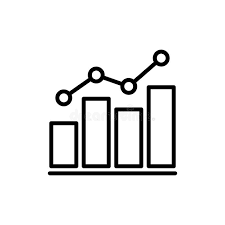
\includegraphics[width=0.5in,height=\textheight,keepaspectratio]{assets/images/analysis.png}\hfill
}{3. Analysis }}\label{analysis}

\subsection{3.1 Exploratory Data
Analysis}\label{exploratory-data-analysis}

At this stage of the analysis, visualizations will be used to explore
the data in more detail, aiming to gain insights into the
characteristics of different variables. To ensure a more structured
analysis process, the datasets will be examined one by one in sequence.
For each dataset, a set of questions will be explored with the aim of
gaining deeper understanding and shedding light on key patterns.

To provide a more detailed analysis of the ``education'' dataset, the
following questions will be examined.

Examining the provinces and years with a high number of individuals
holding higher education degrees or no formal education may offer
meaningful insights into educational disparities.
{\textbf{\emph{Question: Which are the top 10 provinces with the highest
number of university graduates, and which are the top 10 provinces with
the highest number of individuals who have not completed any formal
education?}}}

Based on the graphs presented below, the following observations can be
made:

\begin{itemize}
\item
  The number of individuals with higher education has steadily
  {\textbf{increased}} over the years.
\item
  The provinces with the highest levels of higher education attainment
  remain relatively consistent over time, with major cities such as
  {\textbf{Istanbul}}, {\textbf{Ankara}}, and {\textbf{Izmir}} standing
  out.
\item
  This trend may be attributed to both the larger populations in these
  cities and the higher concentration of universities located there.
\end{itemize}

\begin{Shaded}
\begin{Highlighting}[]
\CommentTok{\#Top 10 Provinces by Higher Education Attainment (Each Year)}
\NormalTok{education }\SpecialCharTok{|\textgreater{}} 
  \FunctionTok{filter}\NormalTok{(Educational\_Status }\SpecialCharTok{==} \StringTok{"Higher Education"}\NormalTok{) }\SpecialCharTok{|\textgreater{}} 
  \FunctionTok{group\_by}\NormalTok{(Year) }\SpecialCharTok{|\textgreater{}} 
  \FunctionTok{slice\_max}\NormalTok{(}\AttributeTok{order\_by =}\NormalTok{ Total, }\AttributeTok{n =} \DecValTok{10}\NormalTok{) }\SpecialCharTok{|\textgreater{}} 
  \FunctionTok{ungroup}\NormalTok{() }\SpecialCharTok{|\textgreater{}} 
  \FunctionTok{ggplot}\NormalTok{(}\FunctionTok{aes}\NormalTok{(}\AttributeTok{x =} \FunctionTok{reorder\_within}\NormalTok{(Province, Total,Year), }\AttributeTok{y =}\NormalTok{ Total }\SpecialCharTok{/} \DecValTok{1000}\NormalTok{,}\AttributeTok{width =} \FloatTok{0.5}\NormalTok{)) }\SpecialCharTok{+}
  \FunctionTok{geom\_bar}\NormalTok{(}\AttributeTok{stat =} \StringTok{"identity"}\NormalTok{, }\AttributeTok{fill =} \StringTok{"orange"}\NormalTok{) }\SpecialCharTok{+}
  \FunctionTok{coord\_flip}\NormalTok{() }\SpecialCharTok{+}
  \FunctionTok{facet\_wrap}\NormalTok{(}\SpecialCharTok{\textasciitilde{}}\NormalTok{Year, }\AttributeTok{scales =} \StringTok{"free\_y"}\NormalTok{) }\SpecialCharTok{+}
  \FunctionTok{scale\_x\_reordered}\NormalTok{() }\SpecialCharTok{+}
  \FunctionTok{labs}\NormalTok{(}
    \AttributeTok{title =} \StringTok{"Top 10 Provinces by Higher Education Attainment (Each Year)"}\NormalTok{,}
    \AttributeTok{x =} \StringTok{"Province"}\NormalTok{,}
    \AttributeTok{y =} \StringTok{"Total (10³)"}
\NormalTok{  ) }\SpecialCharTok{+}
  \FunctionTok{theme\_minimal}\NormalTok{()}\SpecialCharTok{+}
  \FunctionTok{theme}\NormalTok{(}\AttributeTok{axis.text.x =} \FunctionTok{element\_text}\NormalTok{(}\AttributeTok{angle =} \DecValTok{90}\NormalTok{, }\AttributeTok{hjust =} \DecValTok{1}\NormalTok{, }\AttributeTok{size =} \DecValTok{6}\NormalTok{),}\AttributeTok{axis.text.y=} \FunctionTok{element\_text}\NormalTok{(}\AttributeTok{size=}\FloatTok{5.5}\NormalTok{))}
\end{Highlighting}
\end{Shaded}

\pandocbounded{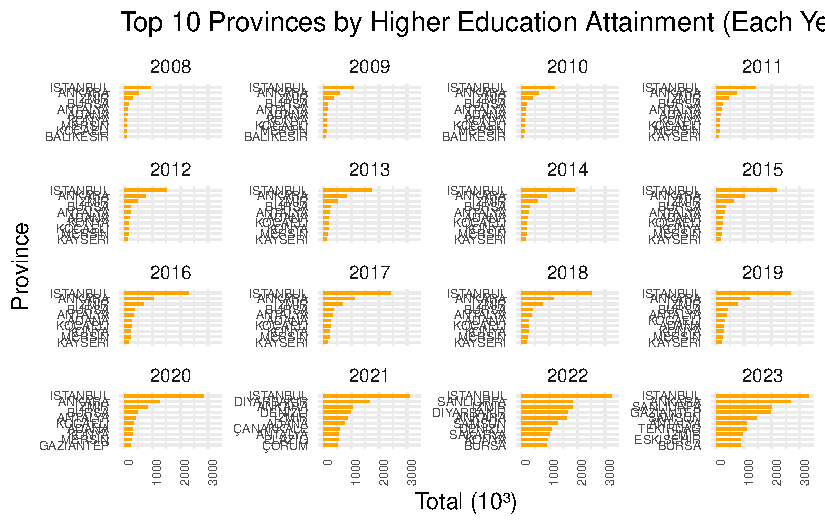
\includegraphics[keepaspectratio]{project_files/figure-pdf/unnamed-chunk-14-1.pdf}}

Based on the graphs presented below, several observations can be made:

\begin{itemize}
\item
  Over the years, the number of individuals with no formal education has
  generally increased, reaching its {\textbf{peak in 2022}} before
  starting to decline.
\item
  The provinces appearing in the top 10 list for individuals with no
  education often overlap with those that also rank high in higher
  education attainment. A major reason for this could be the
  concentration of Turkey's population in these large metropolitan
  areas.
\end{itemize}

\begin{Shaded}
\begin{Highlighting}[]
\NormalTok{education }\SpecialCharTok{|\textgreater{}} 
  \FunctionTok{filter}\NormalTok{(Educational\_Status }\SpecialCharTok{==} \StringTok{"No School Completed"}\NormalTok{) }\SpecialCharTok{|\textgreater{}} 
  \FunctionTok{group\_by}\NormalTok{(Year) }\SpecialCharTok{|\textgreater{}} 
  \FunctionTok{slice\_max}\NormalTok{(}\AttributeTok{order\_by =}\NormalTok{ Total, }\AttributeTok{n =} \DecValTok{10}\NormalTok{) }\SpecialCharTok{|\textgreater{}} 
  \FunctionTok{ungroup}\NormalTok{() }\SpecialCharTok{|\textgreater{}} 
  \FunctionTok{ggplot}\NormalTok{(}\FunctionTok{aes}\NormalTok{(}\AttributeTok{x =} \FunctionTok{reorder\_within}\NormalTok{(Province, Total,Year), }\AttributeTok{y =}\NormalTok{ Total}\SpecialCharTok{/}\DecValTok{1000}\NormalTok{ ,}\AttributeTok{width =} \FloatTok{0.5}\NormalTok{)) }\SpecialCharTok{+}
  \FunctionTok{geom\_bar}\NormalTok{(}\AttributeTok{stat =} \StringTok{"identity"}\NormalTok{, }\AttributeTok{fill =} \StringTok{"darkgreen"}\NormalTok{) }\SpecialCharTok{+}
  \FunctionTok{coord\_flip}\NormalTok{() }\SpecialCharTok{+} 
  \FunctionTok{facet\_wrap}\NormalTok{(}\SpecialCharTok{\textasciitilde{}}\NormalTok{Year, }\AttributeTok{scales =} \StringTok{"free\_y"}\NormalTok{) }\SpecialCharTok{+}
  \FunctionTok{scale\_x\_reordered}\NormalTok{() }\SpecialCharTok{+}
  \FunctionTok{labs}\NormalTok{(}
    \AttributeTok{title =} \StringTok{"Top 10 Provinces by No School Attainment (Each Year)"}\NormalTok{,}
    \AttributeTok{x =} \StringTok{"Province"}\NormalTok{,}
    \AttributeTok{y =} \StringTok{"Total (10³)"}
\NormalTok{  ) }\SpecialCharTok{+}
  \FunctionTok{theme\_minimal}\NormalTok{()}\SpecialCharTok{+}
  \FunctionTok{theme}\NormalTok{(}\AttributeTok{axis.text.x =} \FunctionTok{element\_text}\NormalTok{(}\AttributeTok{angle =} \DecValTok{90}\NormalTok{, }\AttributeTok{hjust =} \DecValTok{1}\NormalTok{, }\AttributeTok{size =} \DecValTok{6}\NormalTok{),}\AttributeTok{axis.text.y=} \FunctionTok{element\_text}\NormalTok{(}\AttributeTok{size=}\FloatTok{5.5}\NormalTok{))}
\end{Highlighting}
\end{Shaded}

\pandocbounded{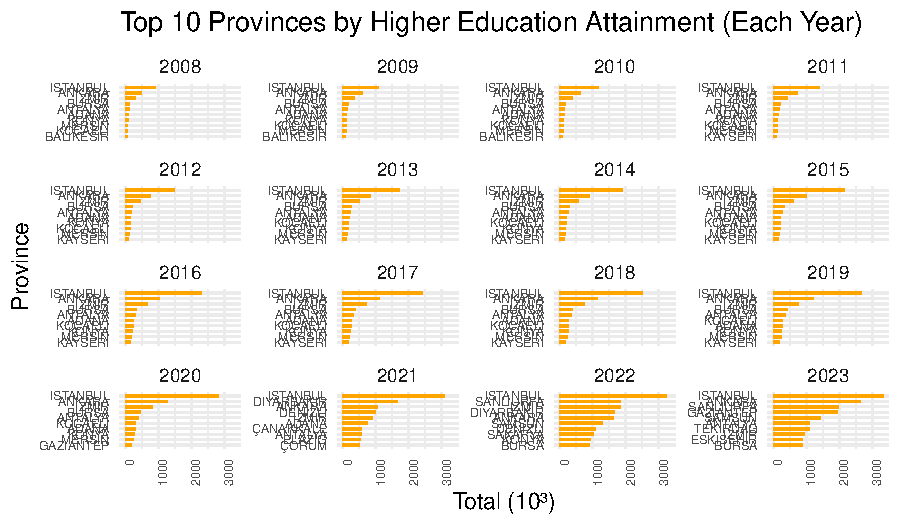
\includegraphics[keepaspectratio]{project_files/figure-pdf/unnamed-chunk-15-1.pdf}}

After examining the number of individuals with no formal education and
those with higher education across provinces, the next step involves
incorporating the gender dimension into the analysis.
{\textbf{\emph{Question: What does the comparison between female and
male proportions tell us about the presumed educational disadvantage
faced by women?}}}

Below, a series of maps illustrate the percentage of women and men with
no formal education across provinces over time. The visualizations show
that, in recent years, the number of {\textbf{men with no education has
begun to surpass that of women}} in many provinces.

Does this observation indicate that the educational disadvantage has
shifted over time to affect men more significantly?

To further investigate the findings from the map above, we can examine
the gender distribution across different education levels (aggregated
for all years at the national level) using the chart below.

Contrary to our earlier observation, the chart reveals that
{\textbf{57.48\%}} of individuals with no formal education are
{\textbf{women}}.

So, what do these seemingly conflicting results actually tell us?

They suggest that, overall, the number of {\textbf{women who have never
received any formal education is significantly higher than that of
men}}, even if recent trends indicate a growing number of uneducated men
in certain regions.

\begin{Shaded}
\begin{Highlighting}[]
\NormalTok{ education }\SpecialCharTok{|\textgreater{}} \FunctionTok{group\_by}\NormalTok{(Educational\_Status)  }\SpecialCharTok{|\textgreater{}}
  \FunctionTok{summarise}\NormalTok{(}\AttributeTok{Male =} \FunctionTok{sum}\NormalTok{(Male),}
            \AttributeTok{Female =} \FunctionTok{sum}\NormalTok{(Female)) }\SpecialCharTok{|\textgreater{}} \FunctionTok{mutate}\NormalTok{(}\AttributeTok{Total =}\NormalTok{ Male }\SpecialCharTok{+}\NormalTok{ Female,}
         \AttributeTok{Male =}\NormalTok{ Male }\SpecialCharTok{/}\NormalTok{ Total }\SpecialCharTok{*} \DecValTok{100}\NormalTok{,}
         \AttributeTok{Female =}\NormalTok{ Female }\SpecialCharTok{/}\NormalTok{ Total }\SpecialCharTok{*} \DecValTok{100}\NormalTok{) }\SpecialCharTok{|\textgreater{}}
  \FunctionTok{pivot\_longer}\NormalTok{(}\AttributeTok{cols =} \FunctionTok{c}\NormalTok{(}\StringTok{"Male"}\NormalTok{, }\StringTok{"Female"}\NormalTok{), }\AttributeTok{names\_to =} \StringTok{"Gender"}\NormalTok{, }\AttributeTok{values\_to =} \StringTok{"Percentage"}\NormalTok{) }\SpecialCharTok{|\textgreater{}}
  \FunctionTok{ggplot}\NormalTok{(}\FunctionTok{aes}\NormalTok{(}\AttributeTok{x =}\NormalTok{ Educational\_Status, }\AttributeTok{y =}\NormalTok{ Percentage, }\AttributeTok{fill =}\NormalTok{ Gender)) }\SpecialCharTok{+}
  \FunctionTok{geom\_bar}\NormalTok{(}\AttributeTok{stat =} \StringTok{"identity"}\NormalTok{, }\AttributeTok{position =} \StringTok{"dodge"}\NormalTok{) }\SpecialCharTok{+}
  \FunctionTok{labs}\NormalTok{(}\AttributeTok{title =} \StringTok{"Educational vs Gender (Country wise)"}\NormalTok{, }\AttributeTok{x =} \StringTok{"Educational Status"}\NormalTok{, }\AttributeTok{y =} \StringTok{"Percentage"}\NormalTok{)}\SpecialCharTok{+}\FunctionTok{geom\_text\_repel}\NormalTok{(}\FunctionTok{aes}\NormalTok{(}\AttributeTok{label =}\FunctionTok{round}\NormalTok{(Percentage,}\DecValTok{2}\NormalTok{)), }\AttributeTok{color =} \StringTok{"black"}\NormalTok{, }\AttributeTok{size =} \FloatTok{3.5}\NormalTok{)}\SpecialCharTok{+}
  \FunctionTok{theme}\NormalTok{(}\AttributeTok{axis.text.x =} \FunctionTok{element\_text}\NormalTok{(}\AttributeTok{angle =} \DecValTok{30}\NormalTok{, }\AttributeTok{hjust =} \DecValTok{1}\NormalTok{, }\AttributeTok{size =} \DecValTok{7}\NormalTok{))}
\end{Highlighting}
\end{Shaded}

\pandocbounded{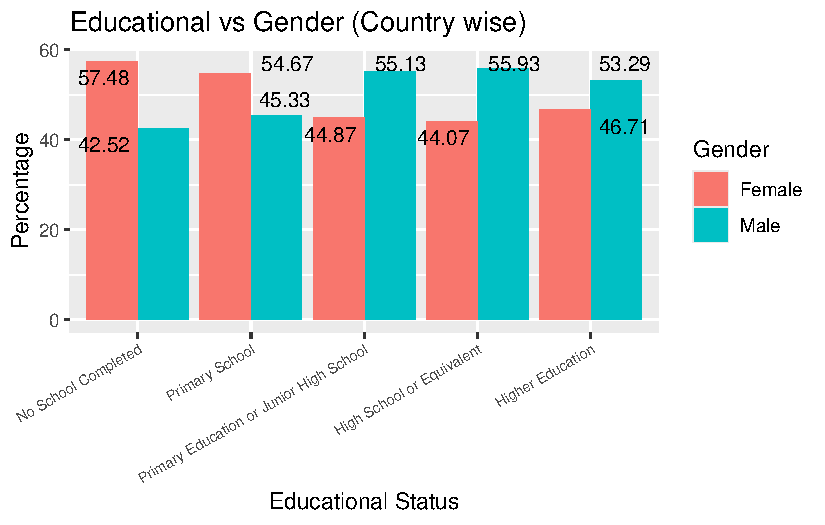
\includegraphics[keepaspectratio]{project_files/figure-pdf/unnamed-chunk-17-1.pdf}}

To provide a more detailed analysis of the ``byeducation'' dataset, the
following questions will be examined.

To closely examine this dataset, the first step is to explore the
relationship between education levels and life satisfaction.
{\textbf{\emph{Question: Which education level group reports higher life
satisfaction, and which one reports the lowest?}}}

Based on the results obtained, the following observations can be made:

\begin{itemize}
\item
  Within a given year, the distribution of education levels across
  happiness categories shows relatively similar proportions.
\item
  Individuals with {\textbf{higher education}} have the
  {\textbf{highest}} average life satisfaction ``Happy'', whereas those
  with only {\textbf{primary school education}} report the
  {\textbf{lowest}}.
\item
  Among those who identify as ``Unhappy,'' the {\textbf{largest
  proportion}} consists of individuals with {\textbf{no formal
  education}}, while the {\textbf{smallest}} share belongs to those with
  {\textbf{higher education}}.
\item
  Individuals with a high school education or with primary/junior high
  school education tend to display similar patterns, showing closely
  aligned averages across the different happiness levels.
\end{itemize}

\begin{Shaded}
\begin{Highlighting}[]
\NormalTok{ byeducation }\SpecialCharTok{|\textgreater{}}
  \FunctionTok{select}\NormalTok{(}\FunctionTok{everything}\NormalTok{()) }\SpecialCharTok{|\textgreater{}}
  \FunctionTok{pivot\_longer}\NormalTok{(}\AttributeTok{cols =} \FunctionTok{c}\NormalTok{(}\StringTok{"No School Completed"}\NormalTok{,}\StringTok{"Primary School"}\NormalTok{,}\StringTok{"Primary Education or Junior High School"}\NormalTok{,}\StringTok{"High School or Equivalent"}\NormalTok{,}\StringTok{"Higher Education"}\NormalTok{), }\AttributeTok{names\_to =} \StringTok{"Education\_Level"}\NormalTok{, }\AttributeTok{values\_to =} \StringTok{"Percentage"}\NormalTok{) }\SpecialCharTok{|\textgreater{}}\FunctionTok{ggplot}\NormalTok{(}\FunctionTok{aes}\NormalTok{(}\AttributeTok{x =}\NormalTok{ Happiness\_Level, }\AttributeTok{y =}\NormalTok{ Percentage, }\AttributeTok{color =}\NormalTok{ Education\_Level)) }\SpecialCharTok{+}
  \FunctionTok{geom\_boxplot}\NormalTok{() }\SpecialCharTok{+}
  \FunctionTok{labs}\NormalTok{(}\AttributeTok{title =} \StringTok{"Happy percentage vs Education Level"}\NormalTok{,}
       \AttributeTok{x =} \StringTok{"Happiness\_Level"}\NormalTok{, }\AttributeTok{y =} \StringTok{"Percentage (\%)"}\NormalTok{, }\AttributeTok{color =} \StringTok{"Education\_Level"}\NormalTok{) }\SpecialCharTok{+}
  \FunctionTok{theme\_minimal}\NormalTok{()}
\end{Highlighting}
\end{Shaded}

\pandocbounded{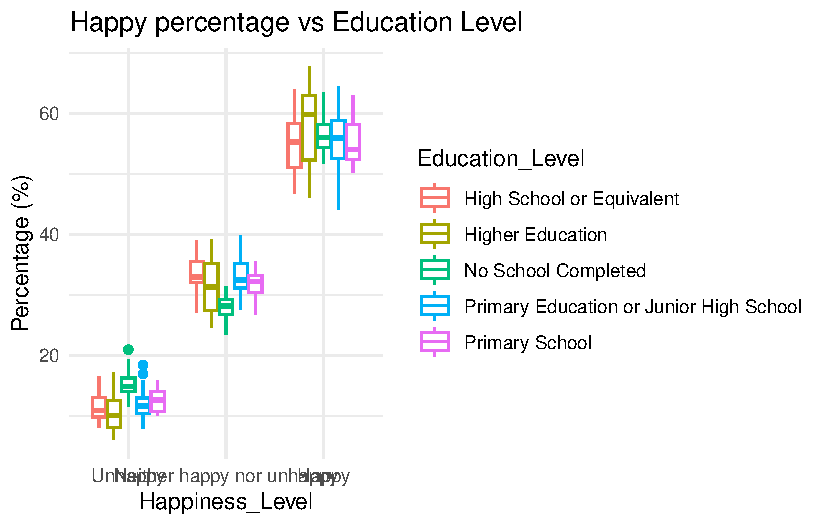
\includegraphics[keepaspectratio]{project_files/figure-pdf/unnamed-chunk-18-1.pdf}}

To provide a more detailed analysis of the ``bygender'' dataset, the
following questions will be examined.

To closely examine the dataset, the first step is to explore the
relationship between education levels and happiness levels.
{\textbf{\emph{Question: How does the percentage of happiness vary for
each gender?}}}

Based on the results obtained, the following observations can be made:

\begin{itemize}
\item
  Within a given year, the distribution of happiness levels across
  genders shows similar proportions for both men and women.
\item
  {\textbf{Women}} report the highest average life satisfaction
  {\textbf{``Happy''}}, while men tend to have the lowest average
  satisfaction.
\item
  The majority of individuals who identify as {\textbf{``Unhappy''}} are
  {\textbf{men}}.
\item
  There is a {\textbf{notable difference}} between the average happiness
  percentages for men and women, particularly at the {\textbf{``Happy''
  level}}.
\end{itemize}

\begin{Shaded}
\begin{Highlighting}[]
\NormalTok{ bygender }\SpecialCharTok{|\textgreater{}} 
  \FunctionTok{select}\NormalTok{( }\FunctionTok{everything}\NormalTok{()) }\SpecialCharTok{|\textgreater{}}
  \FunctionTok{pivot\_longer}\NormalTok{(}\AttributeTok{cols =} \FunctionTok{c}\NormalTok{(}\StringTok{"Male"}\NormalTok{, }\StringTok{"Female"}\NormalTok{), }\AttributeTok{names\_to =} \StringTok{"Gender"}\NormalTok{, }\AttributeTok{values\_to =} \StringTok{"Percentage"}\NormalTok{) }\SpecialCharTok{|\textgreater{}}\FunctionTok{ggplot}\NormalTok{(}\FunctionTok{aes}\NormalTok{(}\AttributeTok{x =}\NormalTok{ Happiness\_Level, }\AttributeTok{y =}\NormalTok{ Percentage, }\AttributeTok{color =}\NormalTok{ Gender)) }\SpecialCharTok{+}
  \FunctionTok{geom\_boxplot}\NormalTok{()}\SpecialCharTok{+}
  \FunctionTok{labs}\NormalTok{(}\AttributeTok{title =} \StringTok{"Happy percentage vs Gender"}\NormalTok{,}
       \AttributeTok{x =} \StringTok{"Happiness\_Level"}\NormalTok{, }\AttributeTok{y =} \StringTok{"Percentage (\%)"}\NormalTok{, }\AttributeTok{color =} \StringTok{"Gender"}\NormalTok{) }\SpecialCharTok{+}
  \FunctionTok{theme\_minimal}\NormalTok{()}
\end{Highlighting}
\end{Shaded}

\pandocbounded{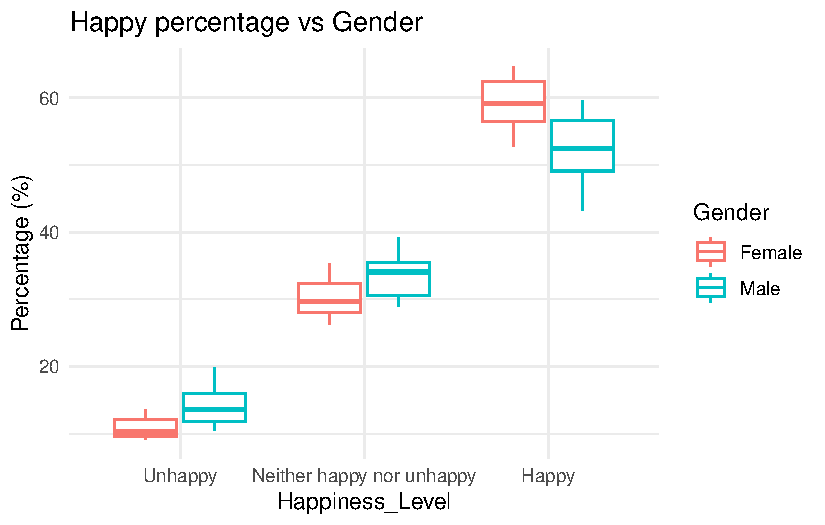
\includegraphics[keepaspectratio]{project_files/figure-pdf/unnamed-chunk-19-1.pdf}}

\subsection{3.2 Trend Analysis}\label{trend-analysis}

In this section, the behavior of different variables within the datasets
over time will be examined. As in previous sections, the datasets will
be analyzed separately, and the time-dependent behavior of the variables
will be explored by addressing various research questions.

\textbf{Analysis for ``education'' dataset}

In the previous sections, we examined the top 10 provinces with the
highest number of university graduates over different years. As the next
step in the analysis, we can investigate the provinces where the rate of
university graduates has increased most rapidly.
{\textbf{\emph{Question: In which provinces has the rate of university
graduates increased most rapidly?}}}

Based on the chart below, the following observations can be made:

\begin{itemize}
\item
  Consistent with our earlier findings, provinces such as Istanbul and
  Ankara, which appeared in the previous analysis, are also among the
  provinces that have shown the fastest growth in the number of
  individuals with higher education. One possible explanation for this
  is the large population size of these cities.
\item
  {\textbf{Istanbul}}, the province with the highest number of
  university graduates, has shown a {\textbf{steady increase between
  2008 and 2023}}. Similarly, {\textbf{Izmir}} has also demonstrated
  consistent growth.
\item
  A particularly noteworthy observation is the {\textbf{sharp upward
  trend in Ankara}}, especially {\textbf{after 2020}}, where the growth
  rate increased significantly. A similar observation can be made for
  {\textbf{Konya}} and {\textbf{Bursa}}, though the growth rate in these
  cities is somewhat slower. This rapid increase, particularly after
  2020, may be attributed to the growth in the number of universities in
  these cities and the migration they have received in recent years.
\end{itemize}

\begin{Shaded}
\begin{Highlighting}[]
\NormalTok{univ\_trend }\OtherTok{\textless{}{-}}\NormalTok{ education }\SpecialCharTok{|\textgreater{}}
  \FunctionTok{filter}\NormalTok{(Educational\_Status }\SpecialCharTok{==} \StringTok{"Higher Education"}\NormalTok{) }\SpecialCharTok{|\textgreater{}}
  \FunctionTok{mutate}\NormalTok{(}\AttributeTok{Total =}\NormalTok{ Male }\SpecialCharTok{+}\NormalTok{ Female)}

\NormalTok{slope\_by\_province }\OtherTok{\textless{}{-}}\NormalTok{ univ\_trend }\SpecialCharTok{\%\textgreater{}\%}
  \FunctionTok{group\_by}\NormalTok{(Province) }\SpecialCharTok{\%\textgreater{}\%}
  \FunctionTok{summarise}\NormalTok{(}\AttributeTok{slope =} \FunctionTok{coef}\NormalTok{(}\FunctionTok{lm}\NormalTok{(Total }\SpecialCharTok{\textasciitilde{}}\NormalTok{ Year))[}\DecValTok{2}\NormalTok{]) }\SpecialCharTok{\%\textgreater{}\%}
  \FunctionTok{arrange}\NormalTok{(}\FunctionTok{desc}\NormalTok{(slope))}

\FunctionTok{head}\NormalTok{(slope\_by\_province, }\DecValTok{10}\NormalTok{)}
\end{Highlighting}
\end{Shaded}

\begin{verbatim}
# A tibble: 10 x 2
   Province    slope
   <chr>       <dbl>
 1 İSTANBUL  166314.
 2 ANKARA     92572.
 3 İZMİR      55971.
 4 BURSA      29044.
 5 KONYA      23179.
 6 ADANA      23058.
 7 KOCAELİ    22834.
 8 ANTALYA    21437.
 9 MERSİN     19919.
10 ESKİŞEHİR  16730.
\end{verbatim}

\begin{Shaded}
\begin{Highlighting}[]
\NormalTok{top\_provinces }\OtherTok{\textless{}{-}}\NormalTok{ slope\_by\_province }\SpecialCharTok{\%\textgreater{}\%}
  \FunctionTok{slice\_max}\NormalTok{(}\AttributeTok{order\_by =}\NormalTok{ slope, }\AttributeTok{n =} \DecValTok{5}\NormalTok{) }\SpecialCharTok{\%\textgreater{}\%}
  \FunctionTok{pull}\NormalTok{(Province)}

\NormalTok{univ\_trend }\SpecialCharTok{\%\textgreater{}\%}
  \FunctionTok{filter}\NormalTok{(Province }\SpecialCharTok{\%in\%}\NormalTok{ top\_provinces) }\SpecialCharTok{\%\textgreater{}\%}
  \FunctionTok{ggplot}\NormalTok{(}\FunctionTok{aes}\NormalTok{(}\AttributeTok{x =}\NormalTok{ Year, }\AttributeTok{y =}\NormalTok{ Total}\SpecialCharTok{/}\DecValTok{1000}\NormalTok{, }\AttributeTok{color =}\NormalTok{ Province, }\AttributeTok{group =}\NormalTok{ Province)) }\SpecialCharTok{+}  
  \FunctionTok{geom\_smooth}\NormalTok{(}\AttributeTok{method =} \StringTok{"loess"}\NormalTok{, }\AttributeTok{se =} \ConstantTok{FALSE}\NormalTok{, }\AttributeTok{linewidth =} \FloatTok{1.2}\NormalTok{) }\SpecialCharTok{+}
  \FunctionTok{labs}\NormalTok{(}\AttributeTok{title =} \StringTok{" Provinces which rate of university graduates increased most rapidly"}\NormalTok{,}
       \AttributeTok{x =} \StringTok{"Year"}\NormalTok{, }\AttributeTok{y =} \StringTok{"Total Graduates (10³) "}\NormalTok{) }\SpecialCharTok{+}
  \FunctionTok{theme\_minimal}\NormalTok{()}
\end{Highlighting}
\end{Shaded}

\begin{verbatim}
`geom_smooth()` using formula = 'y ~ x'
\end{verbatim}

\pandocbounded{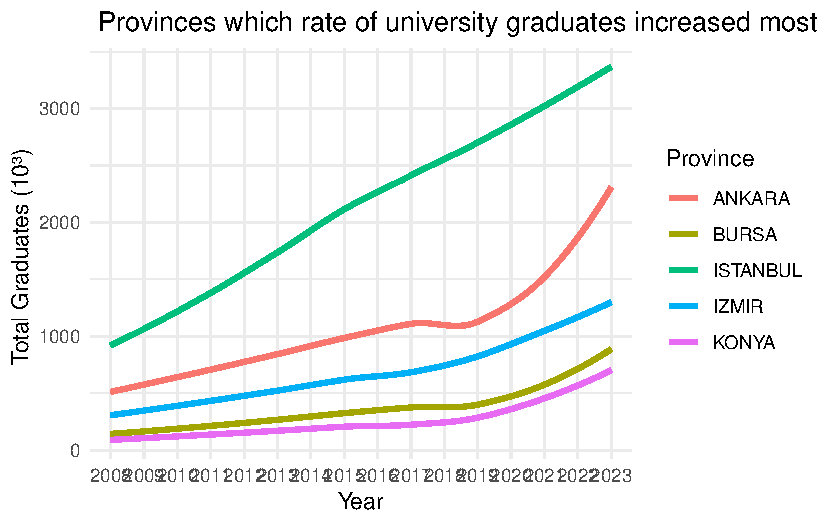
\includegraphics[keepaspectratio]{project_files/figure-pdf/unnamed-chunk-20-1.pdf}}

\textbf{Analysis for ``bygender'' dataset}

In the next step of our analysis, we can consider how life satisfaction
has evolved over time for both men and women, based on the previously
explored relationship between gender and happiness levels.
{\textbf{\emph{Question: How has life satisfaction changed over time for
men and women?}}}

Based on the chart below and in line with our earlier findings, the
following observations can be made:

\begin{itemize}
\item
  It appears that women generally report higher levels of happiness than
  men, supporting the notion that men tend to be more unhappy than
  women.
\item
  In {\textbf{2016}}, a {\textbf{decrease}} was observed in the
  percentage of individuals reporting {\textbf{high life satisfaction}}.
  This decline is mirrored by an {\textbf{increase}} in the percentage
  of individuals identifying as {\textbf{``unhappy''}} after 2016.
\end{itemize}

\begin{Shaded}
\begin{Highlighting}[]
\NormalTok{bygender\_long }\OtherTok{\textless{}{-}}\NormalTok{ bygender }\SpecialCharTok{|\textgreater{}} 
  \FunctionTok{pivot\_longer}\NormalTok{(}\AttributeTok{cols =} \FunctionTok{c}\NormalTok{(}\StringTok{"Male"}\NormalTok{, }\StringTok{"Female"}\NormalTok{), }
               \AttributeTok{names\_to =} \StringTok{"Gender"}\NormalTok{, }
               \AttributeTok{values\_to =} \StringTok{"Percentage"}\NormalTok{)}
\FunctionTok{ggplot}\NormalTok{(bygender\_long, }\FunctionTok{aes}\NormalTok{(}\AttributeTok{x =}\NormalTok{ Year, }\AttributeTok{y =}\NormalTok{ Percentage, }\AttributeTok{color =}\NormalTok{ Gender)) }\SpecialCharTok{+}
  \FunctionTok{geom\_line}\NormalTok{(}\AttributeTok{size =} \FloatTok{1.2}\NormalTok{) }\SpecialCharTok{+}
  \FunctionTok{geom\_point}\NormalTok{(}\AttributeTok{linewidth =} \DecValTok{2}\NormalTok{) }\SpecialCharTok{+}
  \FunctionTok{facet\_wrap}\NormalTok{(}\SpecialCharTok{\textasciitilde{}}\NormalTok{ Happiness\_Level) }\SpecialCharTok{+}
  \FunctionTok{labs}\NormalTok{(}\AttributeTok{title =} \StringTok{"Life Satisfaction Trends by Gender and Level"}\NormalTok{,}
       \AttributeTok{x =} \StringTok{"Year"}\NormalTok{, }\AttributeTok{y =} \StringTok{"Percentage (\%)"}\NormalTok{,}
       \AttributeTok{color =} \StringTok{"Gender"}\NormalTok{) }\SpecialCharTok{+}
  \FunctionTok{theme\_minimal}\NormalTok{()}
\end{Highlighting}
\end{Shaded}

\begin{verbatim}
Warning: Using `size` aesthetic for lines was deprecated in ggplot2 3.4.0.
i Please use `linewidth` instead.
\end{verbatim}

\begin{verbatim}
Warning in geom_point(linewidth = 2): Ignoring unknown parameters: `linewidth`
\end{verbatim}

\pandocbounded{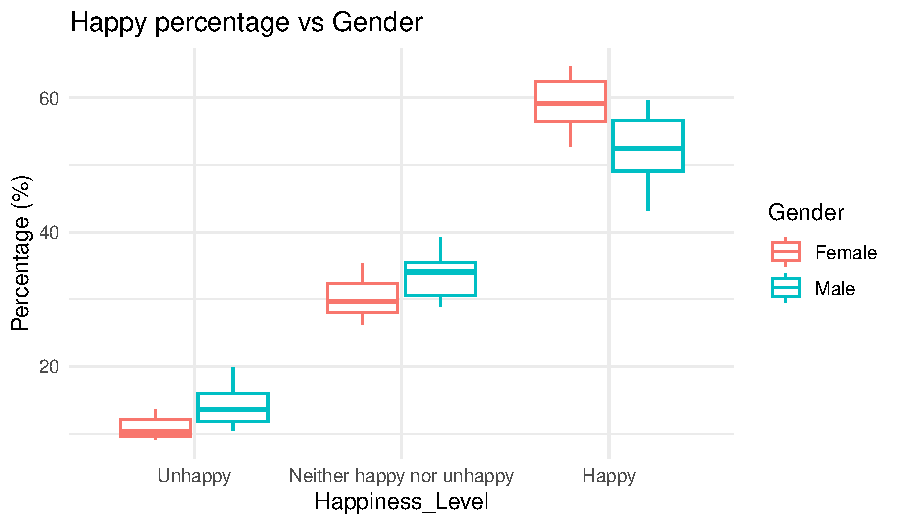
\includegraphics[keepaspectratio]{project_files/figure-pdf/unnamed-chunk-21-1.pdf}}

We can conclude that there is a significant difference between men and
women in terms of happiness levels. This conclusion can be further
developed by examining whether the difference between men and women
persists annually. {\textbf{\emph{Question: Does the difference in life
satisfaction between men and women persist annually?}}}

Based on the analysis below, the following observations can be made:

\begin{itemize}
\item
  {\textbf{Negative values}} indicate that {\textbf{women}} are
  generally {\textbf{happier}} than men.
\item
  When examining the statistical significance of the difference (i.e.,
  whether the {\textbf{difference in happiness between men and women}}
  shows a meaningful trend over time) through linear regression, the
  {\textbf{p-value = 0.046}}, which is less than 0.05, indicating that
  the difference is statistically {\textbf{significant}}. On average,
  the difference between men and women in happiness levels
  {\textbf{decreases by 0.24}} points per year.
\end{itemize}

\begin{Shaded}
\begin{Highlighting}[]
\NormalTok{mutlu\_df }\OtherTok{\textless{}{-}}\NormalTok{ bygender }\SpecialCharTok{|\textgreater{}} 
  \FunctionTok{filter}\NormalTok{(Happiness\_Level }\SpecialCharTok{==} \StringTok{"Happy"}\NormalTok{) }\SpecialCharTok{|\textgreater{}} 
  \FunctionTok{pivot\_longer}\NormalTok{(}\AttributeTok{cols =} \FunctionTok{c}\NormalTok{(Male, Female), }
               \AttributeTok{names\_to =} \StringTok{"Gender"}\NormalTok{, }
               \AttributeTok{values\_to =} \StringTok{"Percentage"}\NormalTok{)}\SpecialCharTok{|\textgreater{}}  
  \FunctionTok{pivot\_wider}\NormalTok{(}\AttributeTok{names\_from =}\NormalTok{ Gender, }\AttributeTok{values\_from =}\NormalTok{ Percentage)}\SpecialCharTok{|\textgreater{}}
  \FunctionTok{mutate}\NormalTok{(}\AttributeTok{Difference =}\NormalTok{ Male }\SpecialCharTok{{-}}\NormalTok{ Female)  }
  
  \FunctionTok{ggplot}\NormalTok{(mutlu\_df, }\FunctionTok{aes}\NormalTok{(}\AttributeTok{x =}\NormalTok{ Year, }\AttributeTok{y =}\NormalTok{ Difference)) }\SpecialCharTok{+}
  \FunctionTok{geom\_line}\NormalTok{(}\AttributeTok{color =} \StringTok{"darkred"}\NormalTok{, }\AttributeTok{size =} \FloatTok{1.2}\NormalTok{) }\SpecialCharTok{+}
  \FunctionTok{geom\_point}\NormalTok{(}\AttributeTok{size =} \DecValTok{2}\NormalTok{, }\AttributeTok{color =} \StringTok{"darkred"}\NormalTok{) }\SpecialCharTok{+}
  \FunctionTok{geom\_hline}\NormalTok{(}\AttributeTok{yintercept =} \DecValTok{0}\NormalTok{, }\AttributeTok{linetype =} \StringTok{"dashed"}\NormalTok{) }\SpecialCharTok{+}
  \FunctionTok{geom\_smooth}\NormalTok{(}\AttributeTok{method =} \StringTok{"lm"}\NormalTok{, }\AttributeTok{se =} \ConstantTok{TRUE}\NormalTok{, }\AttributeTok{color =} \StringTok{"black"}\NormalTok{, }\AttributeTok{linetype =} \StringTok{"dotted"}\NormalTok{) }\SpecialCharTok{+}
  \FunctionTok{labs}\NormalTok{(}\AttributeTok{title =} \StringTok{"Trend of Gender Difference in Happiness Over Time"}\NormalTok{,}
       \AttributeTok{subtitle =} \StringTok{"Black dotted line: linear trend"}\NormalTok{,}
       \AttributeTok{x =} \StringTok{"Year"}\NormalTok{, }\AttributeTok{y =} \StringTok{"Happiness Difference (Male {-} Female)"}\NormalTok{) }\SpecialCharTok{+}
  \FunctionTok{theme\_minimal}\NormalTok{()}
\end{Highlighting}
\end{Shaded}

\begin{verbatim}
`geom_smooth()` using formula = 'y ~ x'
\end{verbatim}

\pandocbounded{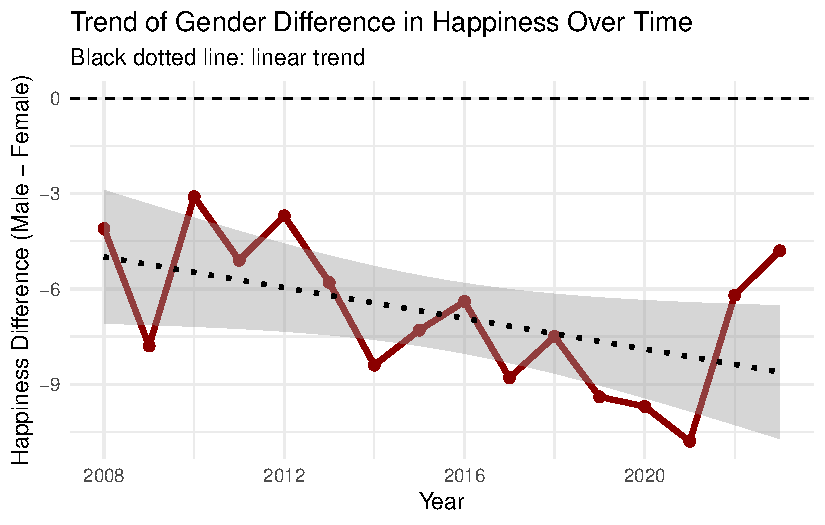
\includegraphics[keepaspectratio]{project_files/figure-pdf/unnamed-chunk-22-1.pdf}}

\begin{Shaded}
\begin{Highlighting}[]
\NormalTok{model }\OtherTok{\textless{}{-}} \FunctionTok{lm}\NormalTok{(Difference }\SpecialCharTok{\textasciitilde{}}\NormalTok{ Year, }\AttributeTok{data =}\NormalTok{ mutlu\_df)}
\FunctionTok{summary}\NormalTok{(model)}
\end{Highlighting}
\end{Shaded}

\begin{verbatim}

Call:
lm(formula = Difference ~ Year, data = mutlu_df)

Residuals:
    Min      1Q  Median      3Q     Max 
-2.6632 -1.7616  0.1562  1.2136  3.8206 

Coefficients:
            Estimate Std. Error t value Pr(>|t|)  
(Intercept) 480.7669   223.5764   2.150   0.0495 *
Year         -0.2419     0.1109  -2.181   0.0468 *
---
Signif. codes:  0 '***' 0.001 '**' 0.01 '*' 0.05 '.' 0.1 ' ' 1

Residual standard error: 2.045 on 14 degrees of freedom
Multiple R-squared:  0.2536,    Adjusted R-squared:  0.2003 
F-statistic: 4.756 on 1 and 14 DF,  p-value: 0.04675
\end{verbatim}

Similarly, the difference in happiness levels between men and women at
the {\textbf{``Unhappy'' level}} has also been examined for statistical
{\textbf{significance}}. According to the results, since {\textbf{p =
0.0268}}, which is less than 0.05, the difference is statistically
significant. On average, the difference between men and women in the
``Unhappy'' category {\textbf{increases by 0.17}} points per year.

\begin{Shaded}
\begin{Highlighting}[]
\NormalTok{mutsuz\_df }\OtherTok{\textless{}{-}}\NormalTok{ bygender }\SpecialCharTok{|\textgreater{}} 
  \FunctionTok{filter}\NormalTok{(Happiness\_Level }\SpecialCharTok{==} \StringTok{"Unhappy"}\NormalTok{) }\SpecialCharTok{|\textgreater{}} 
  \FunctionTok{pivot\_longer}\NormalTok{(}\AttributeTok{cols =} \FunctionTok{c}\NormalTok{(Male, Female), }
               \AttributeTok{names\_to =} \StringTok{"Gender"}\NormalTok{, }
               \AttributeTok{values\_to =} \StringTok{"Percentage"}\NormalTok{)}\SpecialCharTok{|\textgreater{}}  
  \FunctionTok{pivot\_wider}\NormalTok{(}\AttributeTok{names\_from =}\NormalTok{ Gender, }\AttributeTok{values\_from =}\NormalTok{ Percentage)}\SpecialCharTok{|\textgreater{}}
  \FunctionTok{mutate}\NormalTok{(}\AttributeTok{Difference =}\NormalTok{ Male }\SpecialCharTok{{-}}\NormalTok{ Female)  }
  
  \FunctionTok{ggplot}\NormalTok{(mutsuz\_df, }\FunctionTok{aes}\NormalTok{(}\AttributeTok{x =}\NormalTok{ Year, }\AttributeTok{y =}\NormalTok{ Difference)) }\SpecialCharTok{+}
  \FunctionTok{geom\_line}\NormalTok{(}\AttributeTok{color =} \StringTok{"darkred"}\NormalTok{, }\AttributeTok{size =} \FloatTok{1.2}\NormalTok{) }\SpecialCharTok{+}
  \FunctionTok{geom\_point}\NormalTok{(}\AttributeTok{size =} \DecValTok{2}\NormalTok{, }\AttributeTok{color =} \StringTok{"darkred"}\NormalTok{) }\SpecialCharTok{+}
  \FunctionTok{geom\_hline}\NormalTok{(}\AttributeTok{yintercept =} \DecValTok{0}\NormalTok{, }\AttributeTok{linetype =} \StringTok{"dashed"}\NormalTok{) }\SpecialCharTok{+}
  \FunctionTok{geom\_smooth}\NormalTok{(}\AttributeTok{method =} \StringTok{"lm"}\NormalTok{, }\AttributeTok{se =} \ConstantTok{TRUE}\NormalTok{, }\AttributeTok{color =} \StringTok{"black"}\NormalTok{, }\AttributeTok{linetype =} \StringTok{"dotted"}\NormalTok{) }\SpecialCharTok{+}
  \FunctionTok{labs}\NormalTok{(}\AttributeTok{title =} \StringTok{"Trend of Gender Difference in Unhappiness Over Time"}\NormalTok{,}
       \AttributeTok{subtitle =} \StringTok{"Black dotted line: linear trend"}\NormalTok{,}
       \AttributeTok{x =} \StringTok{"Year"}\NormalTok{, }\AttributeTok{y =} \StringTok{"Happiness Difference (Male {-} Female)"}\NormalTok{) }\SpecialCharTok{+}
  \FunctionTok{theme\_minimal}\NormalTok{()}
\end{Highlighting}
\end{Shaded}

\begin{verbatim}
`geom_smooth()` using formula = 'y ~ x'
\end{verbatim}

\pandocbounded{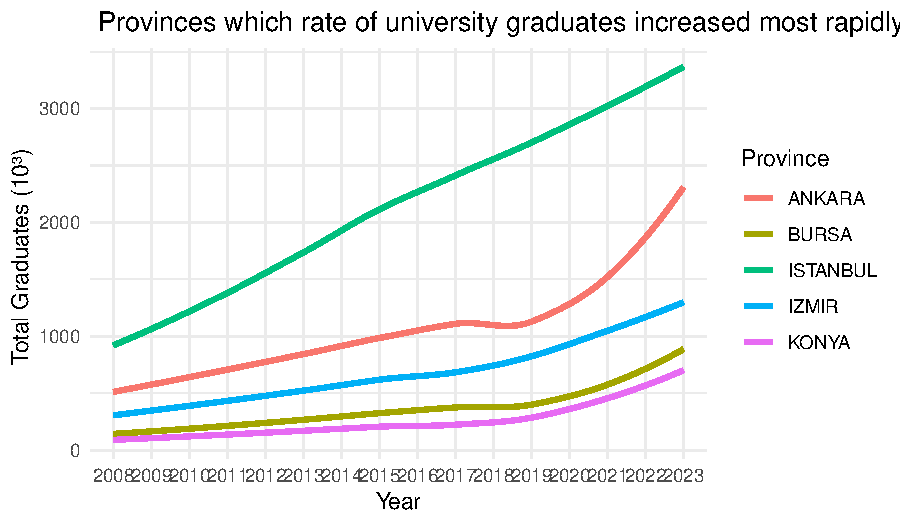
\includegraphics[keepaspectratio]{project_files/figure-pdf/unnamed-chunk-23-1.pdf}}

\begin{Shaded}
\begin{Highlighting}[]
\NormalTok{model }\OtherTok{\textless{}{-}} \FunctionTok{lm}\NormalTok{(Difference }\SpecialCharTok{\textasciitilde{}}\NormalTok{ Year, }\AttributeTok{data =}\NormalTok{ mutsuz\_df)}
\FunctionTok{summary}\NormalTok{(model)}
\end{Highlighting}
\end{Shaded}

\begin{verbatim}

Call:
lm(formula = Difference ~ Year, data = mutsuz_df)

Residuals:
    Min      1Q  Median      3Q     Max 
-1.4704 -0.8468 -0.5268  0.6701  2.4760 

Coefficients:
              Estimate Std. Error t value Pr(>|t|)  
(Intercept) -345.70574  141.18345  -2.449   0.0281 *
Year           0.17324    0.07005   2.473   0.0268 *
---
Signif. codes:  0 '***' 0.001 '**' 0.01 '*' 0.05 '.' 0.1 ' ' 1

Residual standard error: 1.292 on 14 degrees of freedom
Multiple R-squared:  0.304, Adjusted R-squared:  0.2543 
F-statistic: 6.116 on 1 and 14 DF,  p-value: 0.02683
\end{verbatim}

\textbf{Analysis for ``byeducation'' dataset}

We have previously gathered some insights regarding the relationship
between education levels and happiness levels in the dataset. As the
next step in this analysis, we can consider how life satisfaction has
evolved over time for different education levels.
{\textbf{\emph{Question: How has life satisfaction percentage changed
over level of education?}}}

Based on the analysis provided below, the following observations can be
made:

\begin{itemize}
\item
  The percentage of individuals who report being {\textbf{happy}} has
  {\textbf{decreased across all education levels}} over time.
\item
  The {\textbf{smallest decrease}} in happiness levels has been observed
  among individuals {\textbf{without any education}}, with an average
  decrease of just {\textbf{0.0089}}, which is a very low rate.
\item
  The education level with the {\textbf{greatest decline}} in life
  satisfaction over time is among individuals with {\textbf{higher
  education}}. For this group, the happiness percentage has decreased by
  an average of {\textbf{1.369}} points per year.
\end{itemize}

\begin{Shaded}
\begin{Highlighting}[]
\NormalTok{edu\_happy }\OtherTok{\textless{}{-}}\NormalTok{ byeducation }\SpecialCharTok{|\textgreater{}}
  \FunctionTok{filter}\NormalTok{(Happiness\_Level}\SpecialCharTok{==}\StringTok{"Happy"}\NormalTok{)}\SpecialCharTok{|\textgreater{}}\FunctionTok{pivot\_longer}\NormalTok{(}\FunctionTok{c}\NormalTok{(}\StringTok{\textasciigrave{}}\AttributeTok{No School Completed}\StringTok{\textasciigrave{}}\NormalTok{,}\StringTok{\textasciigrave{}}\AttributeTok{Primary School}\StringTok{\textasciigrave{}}\NormalTok{,}\StringTok{\textasciigrave{}}\AttributeTok{Primary Education or Junior High School}\StringTok{\textasciigrave{}}\NormalTok{,}\StringTok{\textasciigrave{}}\AttributeTok{High School or Equivalent}\StringTok{\textasciigrave{}}\NormalTok{,}\StringTok{\textasciigrave{}}\AttributeTok{Higher Education}\StringTok{\textasciigrave{}}\NormalTok{),}
               \AttributeTok{names\_to  =} \StringTok{"Educational\_Status"}\NormalTok{,}
               \AttributeTok{values\_to =} \StringTok{"Percentage"}\NormalTok{) }

\NormalTok{edu\_happy}\SpecialCharTok{$}\NormalTok{Educational\_Status }\OtherTok{\textless{}{-}} \FunctionTok{factor}\NormalTok{(}
\NormalTok{  edu\_happy}\SpecialCharTok{$}\NormalTok{Educational\_Status,}
  \AttributeTok{levels =} \FunctionTok{c}\NormalTok{(}\StringTok{"No School Completed"}\NormalTok{,}\StringTok{"Primary School"}\NormalTok{,}\StringTok{"Primary Education or Junior High School"}\NormalTok{,}\StringTok{"High School or Equivalent"}\NormalTok{,}\StringTok{"Higher Education"}\NormalTok{,}\AttributeTok{order=}\ConstantTok{TRUE}\NormalTok{)}
\NormalTok{)}

\NormalTok{edu\_trends }\OtherTok{\textless{}{-}}\NormalTok{ edu\_happy }\SpecialCharTok{\%\textgreater{}\%}
  \FunctionTok{group\_by}\NormalTok{(Educational\_Status) }\SpecialCharTok{\%\textgreater{}\%}
  \FunctionTok{do}\NormalTok{(}\FunctionTok{tidy}\NormalTok{(}\FunctionTok{lm}\NormalTok{(Percentage }\SpecialCharTok{\textasciitilde{}}\NormalTok{ Year, }\AttributeTok{data =}\NormalTok{ .))) }\SpecialCharTok{\%\textgreater{}\%}
  \FunctionTok{filter}\NormalTok{(term }\SpecialCharTok{==} \StringTok{"Year"}\NormalTok{) }\SpecialCharTok{\%\textgreater{}\%}
  \FunctionTok{arrange}\NormalTok{(}\FunctionTok{desc}\NormalTok{(estimate))}

\NormalTok{edu\_trends }\SpecialCharTok{|\textgreater{}} \FunctionTok{kbl}\NormalTok{() }\SpecialCharTok{|\textgreater{}} \FunctionTok{kable\_styling}\NormalTok{()}
\end{Highlighting}
\end{Shaded}

\begin{table}
\centering
\begin{tabular}[t]{l|l|r|r|r|r}
\hline
Educational\_Status & term & estimate & std.error & statistic & p.value\\
\hline
No School Completed & Year & -0.0882828 & 0.1888264 & -0.4675341 & 0.6473120\\
\hline
Primary School & Year & -0.3969668 & 0.1949510 & -2.0362384 & 0.0611031\\
\hline
High School or Equivalent & Year & -0.8323926 & 0.2130358 & -3.9072905 & 0.0015789\\
\hline
Primary Education or Junior High School & Year & -0.8840392 & 0.2311315 & -3.8248326 & 0.0018575\\
\hline
Higher Education & Year & -1.3692589 & 0.1712698 & -7.9947499 & 0.0000014\\
\hline
\end{tabular}
\end{table}

\begin{Shaded}
\begin{Highlighting}[]
\FunctionTok{ggplot}\NormalTok{(edu\_happy, }\FunctionTok{aes}\NormalTok{(}\AttributeTok{x =}\NormalTok{ Year, }\AttributeTok{y =}\NormalTok{ Percentage, }\AttributeTok{color =}\NormalTok{ Educational\_Status)) }\SpecialCharTok{+}
  \FunctionTok{geom\_line}\NormalTok{() }\SpecialCharTok{+}
  \FunctionTok{labs}\NormalTok{(}\AttributeTok{title =} \StringTok{"Happiness Trend by Education Level Over Years"}\NormalTok{)}\SpecialCharTok{+}
  \FunctionTok{theme\_minimal}\NormalTok{()}
\end{Highlighting}
\end{Shaded}

\pandocbounded{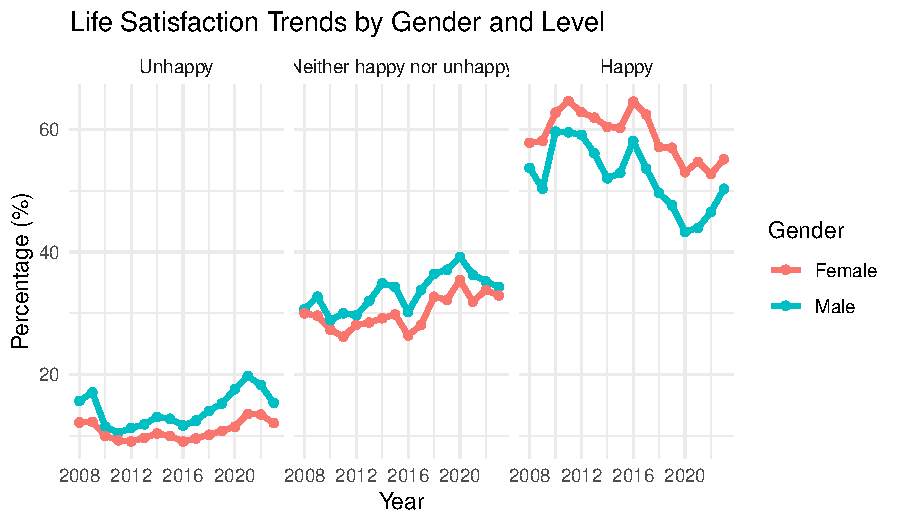
\includegraphics[keepaspectratio]{project_files/figure-pdf/unnamed-chunk-24-1.pdf}}

\begin{Shaded}
\begin{Highlighting}[]
\FunctionTok{ggplot}\NormalTok{(edu\_happy, }\FunctionTok{aes}\NormalTok{(}\AttributeTok{x =}\NormalTok{ Year, }\AttributeTok{y =}\NormalTok{ Percentage, }\AttributeTok{color =}\NormalTok{ Educational\_Status)) }\SpecialCharTok{+}
 \FunctionTok{geom\_point}\NormalTok{() }\SpecialCharTok{+}
  \FunctionTok{geom\_smooth}\NormalTok{(}\AttributeTok{method =} \StringTok{"lm"}\NormalTok{, }\AttributeTok{se =} \ConstantTok{FALSE}\NormalTok{, }\AttributeTok{size =} \FloatTok{1.2}\NormalTok{) }\SpecialCharTok{+}
  \FunctionTok{labs}\NormalTok{(}\AttributeTok{title =} \StringTok{"Life satisfaction percentage changed over level of education"}\NormalTok{,}
       \AttributeTok{x =} \StringTok{"Year"}\NormalTok{, }\AttributeTok{y =} \StringTok{"Happy (\%)"}\NormalTok{) }\SpecialCharTok{+}
  \FunctionTok{theme\_minimal}\NormalTok{()}
\end{Highlighting}
\end{Shaded}

\begin{verbatim}
`geom_smooth()` using formula = 'y ~ x'
\end{verbatim}

\pandocbounded{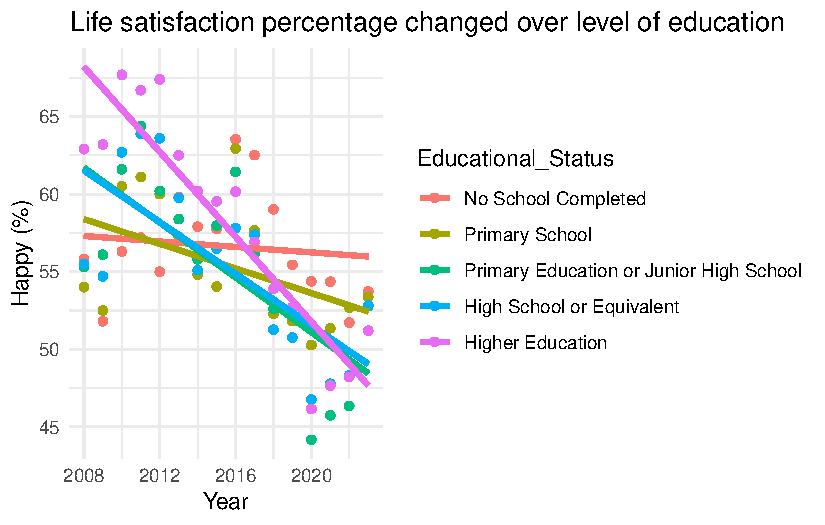
\includegraphics[keepaspectratio]{project_files/figure-pdf/unnamed-chunk-24-2.pdf}}

The same analysis has been conducted for the ``Unhappy'' happiness
level, and the following results were found:

\begin{itemize}
\item
  The percentage of individuals who identify as {\textbf{``Unhappy''}}
  has {\textbf{increased}} over time for all education levels,
  {\textbf{except for those without any education}}.
\item
  For individuals {\textbf{without any education}}, the percentage of
  those who identify as ``Unhappy'' has decreased over time, with an
  average {\textbf{decrease of 0.065}} per year.
\item
  The education level with the {\textbf{largest increase}} in the
  percentage of individuals who identify as {\textbf{``Unhappy'' over
  time is higher education}}. For this group, the percentage of those
  who report being ``Unhappy'' has increased by an average of
  {\textbf{0.45}} points per year.
\end{itemize}

\begin{Shaded}
\begin{Highlighting}[]
\NormalTok{edu\_unhappy }\OtherTok{\textless{}{-}}\NormalTok{ byeducation }\SpecialCharTok{|\textgreater{}}
  \FunctionTok{filter}\NormalTok{(Happiness\_Level}\SpecialCharTok{==}\StringTok{"Unhappy"}\NormalTok{)}\SpecialCharTok{|\textgreater{}}\FunctionTok{pivot\_longer}\NormalTok{(}\FunctionTok{c}\NormalTok{(}\StringTok{\textasciigrave{}}\AttributeTok{No School Completed}\StringTok{\textasciigrave{}}\NormalTok{,}\StringTok{\textasciigrave{}}\AttributeTok{Primary School}\StringTok{\textasciigrave{}}\NormalTok{,}\StringTok{\textasciigrave{}}\AttributeTok{Primary Education or Junior High School}\StringTok{\textasciigrave{}}\NormalTok{,}\StringTok{\textasciigrave{}}\AttributeTok{High School or Equivalent}\StringTok{\textasciigrave{}}\NormalTok{,}\StringTok{\textasciigrave{}}\AttributeTok{Higher Education}\StringTok{\textasciigrave{}}\NormalTok{),}
               \AttributeTok{names\_to  =} \StringTok{"Educational\_Status"}\NormalTok{,}
               \AttributeTok{values\_to =} \StringTok{"Percentage"}\NormalTok{) }

\NormalTok{edu\_unhappy}\SpecialCharTok{$}\NormalTok{Educational\_Status }\OtherTok{\textless{}{-}} \FunctionTok{factor}\NormalTok{(}
\NormalTok{  edu\_unhappy}\SpecialCharTok{$}\NormalTok{Educational\_Status,}
  \AttributeTok{levels =} \FunctionTok{c}\NormalTok{(}\StringTok{"No School Completed"}\NormalTok{,}\StringTok{"Primary School"}\NormalTok{,}\StringTok{"Primary Education or Junior High School"}\NormalTok{,}\StringTok{"High School or Equivalent"}\NormalTok{,}\StringTok{"Higher Education"}\NormalTok{,}\AttributeTok{order=}\ConstantTok{TRUE}\NormalTok{)}
\NormalTok{)}

\NormalTok{edu\_trends }\OtherTok{\textless{}{-}}\NormalTok{ edu\_unhappy }\SpecialCharTok{\%\textgreater{}\%}
  \FunctionTok{group\_by}\NormalTok{(Educational\_Status) }\SpecialCharTok{\%\textgreater{}\%}
  \FunctionTok{do}\NormalTok{(}\FunctionTok{tidy}\NormalTok{(}\FunctionTok{lm}\NormalTok{(Percentage }\SpecialCharTok{\textasciitilde{}}\NormalTok{ Year, }\AttributeTok{data =}\NormalTok{ .))) }\SpecialCharTok{\%\textgreater{}\%}
  \FunctionTok{filter}\NormalTok{(term }\SpecialCharTok{==} \StringTok{"Year"}\NormalTok{) }\SpecialCharTok{\%\textgreater{}\%}
  \FunctionTok{arrange}\NormalTok{(}\FunctionTok{desc}\NormalTok{(estimate))}

\NormalTok{edu\_trends }\SpecialCharTok{|\textgreater{}} \FunctionTok{kbl}\NormalTok{() }\SpecialCharTok{|\textgreater{}} \FunctionTok{kable\_styling}\NormalTok{()}
\end{Highlighting}
\end{Shaded}

\begin{table}
\centering
\begin{tabular}[t]{l|l|r|r|r|r}
\hline
Educational\_Status & term & estimate & std.error & statistic & p.value\\
\hline
Higher Education & Year & 0.4521631 & 0.1235502 & 3.6597527 & 0.0025746\\
\hline
Primary Education or Junior High School & Year & 0.3733905 & 0.1286275 & 2.9028818 & 0.0115759\\
\hline
High School or Equivalent & Year & 0.3401795 & 0.1121412 & 3.0334923 & 0.0089378\\
\hline
Primary School & Year & 0.1823240 & 0.0966591 & 1.8862576 & 0.0801774\\
\hline
No School Completed & Year & -0.0656706 & 0.1318412 & -0.4981037 & 0.6261441\\
\hline
\end{tabular}
\end{table}

\begin{Shaded}
\begin{Highlighting}[]
\FunctionTok{ggplot}\NormalTok{(edu\_unhappy, }\FunctionTok{aes}\NormalTok{(}\AttributeTok{x =}\NormalTok{ Year, }\AttributeTok{y =}\NormalTok{ Percentage, }\AttributeTok{color =}\NormalTok{ Educational\_Status)) }\SpecialCharTok{+}
  \FunctionTok{geom\_line}\NormalTok{() }\SpecialCharTok{+}
  \FunctionTok{labs}\NormalTok{(}\AttributeTok{title =} \StringTok{"Unhappiness Trend by Education Level Over Years"}\NormalTok{)}\SpecialCharTok{+}
  \FunctionTok{theme\_minimal}\NormalTok{()}
\end{Highlighting}
\end{Shaded}

\pandocbounded{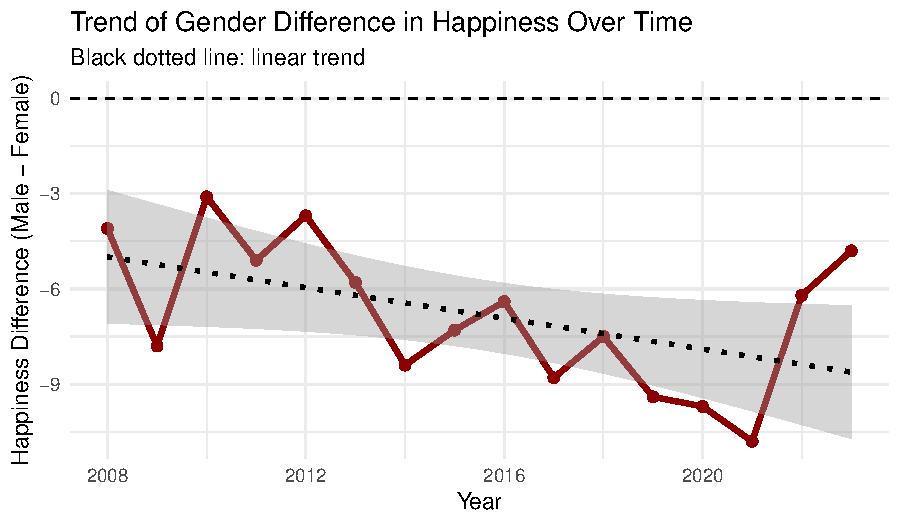
\includegraphics[keepaspectratio]{project_files/figure-pdf/unnamed-chunk-25-1.pdf}}

\begin{Shaded}
\begin{Highlighting}[]
\FunctionTok{ggplot}\NormalTok{(edu\_unhappy, }\FunctionTok{aes}\NormalTok{(}\AttributeTok{x =}\NormalTok{ Year, }\AttributeTok{y =}\NormalTok{ Percentage, }\AttributeTok{color =}\NormalTok{ Educational\_Status)) }\SpecialCharTok{+}
 \FunctionTok{geom\_point}\NormalTok{() }\SpecialCharTok{+}
  \FunctionTok{geom\_smooth}\NormalTok{(}\AttributeTok{method =} \StringTok{"lm"}\NormalTok{, }\AttributeTok{se =} \ConstantTok{FALSE}\NormalTok{, }\AttributeTok{size =} \FloatTok{1.2}\NormalTok{) }\SpecialCharTok{+}
  \FunctionTok{labs}\NormalTok{(}\AttributeTok{title =} \StringTok{"Life satisfaction  percentage changed over level of education"}\NormalTok{,}
       \AttributeTok{x =} \StringTok{"Year"}\NormalTok{, }\AttributeTok{y =} \StringTok{"Unhappy (\%)"}\NormalTok{) }\SpecialCharTok{+}
  \FunctionTok{theme\_minimal}\NormalTok{()}
\end{Highlighting}
\end{Shaded}

\begin{verbatim}
`geom_smooth()` using formula = 'y ~ x'
\end{verbatim}

\pandocbounded{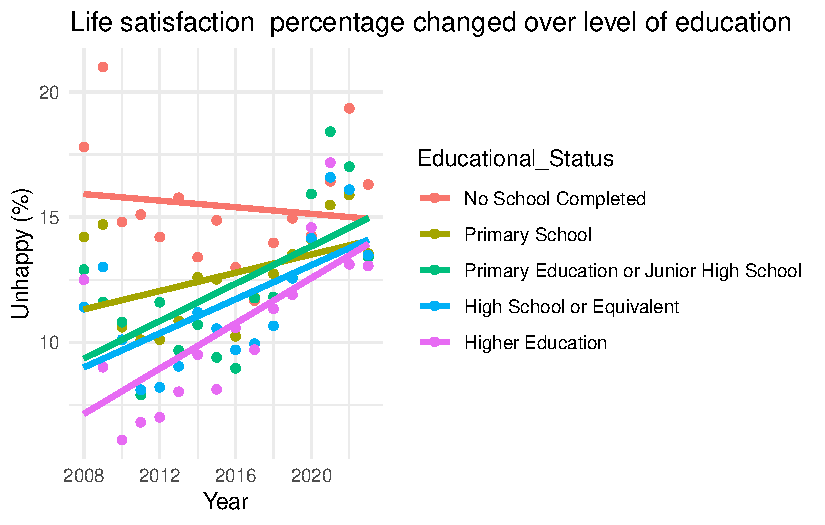
\includegraphics[keepaspectratio]{project_files/figure-pdf/unnamed-chunk-25-2.pdf}}

\subsection{3.3 Model Fitting}\label{model-fitting}

In this section, the primary objective of the research will be addressed
by statistically examining the relationships between variables that
influence individuals' happiness levels, their interconnections, and
their association with happiness levels in more detail. Based on the
findings, predictive models for the future will be developed. This
approach will be carried out, as in previous steps, by answering key
questions.

\begin{itemize}
\tightlist
\item
  {\textbf{\emph{Question: Is there a significant difference between
  educational level and happiness level? (using the ``byeducation''
  dataset)}}}
\end{itemize}

According to the Chi-square test{[}3{]}, the {\textbf{p-value is
2.2e-16}}, which is less than 0.05. Therefore, it can be concluded that
happiness levels are {\textbf{significantly}} associated with
{\textbf{education level}}.

\begin{Shaded}
\begin{Highlighting}[]
\CommentTok{\#}
\NormalTok{df}\OtherTok{\textless{}{-}}\NormalTok{ byeducation }\SpecialCharTok{|\textgreater{}} \FunctionTok{pivot\_longer}\NormalTok{(}\FunctionTok{c}\NormalTok{(}\StringTok{\textasciigrave{}}\AttributeTok{No School Completed}\StringTok{\textasciigrave{}}\NormalTok{,}\StringTok{\textasciigrave{}}\AttributeTok{Primary School}\StringTok{\textasciigrave{}}\NormalTok{,}\StringTok{\textasciigrave{}}\AttributeTok{Primary Education or Junior High School}\StringTok{\textasciigrave{}}\NormalTok{,}\StringTok{\textasciigrave{}}\AttributeTok{High School or Equivalent}\StringTok{\textasciigrave{}}\NormalTok{,}\StringTok{\textasciigrave{}}\AttributeTok{Higher Education}\StringTok{\textasciigrave{}}\NormalTok{),}
               \AttributeTok{names\_to  =} \StringTok{"Educational\_Status"}\NormalTok{,}
               \AttributeTok{values\_to =} \StringTok{"Percentage"}\NormalTok{) }\SpecialCharTok{|\textgreater{}}
 \FunctionTok{mutate}\NormalTok{(}\AttributeTok{Estimated\_Count =} \FunctionTok{round}\NormalTok{(Percentage }\SpecialCharTok{*} \DecValTok{1000} \SpecialCharTok{/} \DecValTok{100}\NormalTok{))}
 

\NormalTok{summary\_table }\OtherTok{\textless{}{-}}\NormalTok{ df }\SpecialCharTok{\%\textgreater{}\%}
  \FunctionTok{group\_by}\NormalTok{(Happiness\_Level, Educational\_Status) }\SpecialCharTok{\%\textgreater{}\%}
  \FunctionTok{summarise}\NormalTok{(}\AttributeTok{Count =} \FunctionTok{sum}\NormalTok{(Estimated\_Count), }\AttributeTok{.groups =} \StringTok{"drop"}\NormalTok{)}

\NormalTok{contingency\_matrix }\OtherTok{\textless{}{-}}\NormalTok{ summary\_table }\SpecialCharTok{\%\textgreater{}\%}
  \FunctionTok{pivot\_wider}\NormalTok{(}\AttributeTok{names\_from =}\NormalTok{ Happiness\_Level, }\AttributeTok{values\_from =}\NormalTok{ Count) }\SpecialCharTok{\%\textgreater{}\%}
  \FunctionTok{column\_to\_rownames}\NormalTok{(}\StringTok{"Educational\_Status"}\NormalTok{) }\SpecialCharTok{\%\textgreater{}\%}
  \FunctionTok{as.matrix}\NormalTok{()}
\FunctionTok{chisq.test}\NormalTok{(contingency\_matrix)}
\end{Highlighting}
\end{Shaded}

\begin{verbatim}

    Pearson's Chi-squared test

data:  contingency_matrix
X-squared = 277.05, df = 8, p-value < 2.2e-16
\end{verbatim}

\begin{itemize}
\tightlist
\item
  {\textbf{\emph{Question: Is there a significant difference between
  gender and happiness level? (using the ``bygender'' dataset)}}}
\end{itemize}

According to the Chi-square test, the {\textbf{p-value is 2.2e-16}},
which is less than 0.05. Therefore, it can be concluded that happiness
levels are {\textbf{significantly}} associated with {\textbf{gender}}.

\begin{Shaded}
\begin{Highlighting}[]
\CommentTok{\#}
\NormalTok{df1}\OtherTok{\textless{}{-}}\NormalTok{ bygender }\SpecialCharTok{|\textgreater{}} \FunctionTok{pivot\_longer}\NormalTok{(}\FunctionTok{c}\NormalTok{(Male,Female),}
               \AttributeTok{names\_to  =} \StringTok{"Gender"}\NormalTok{,}
               \AttributeTok{values\_to =} \StringTok{"Percentage"}\NormalTok{) }\SpecialCharTok{|\textgreater{}}
 \FunctionTok{mutate}\NormalTok{(}\AttributeTok{Estimated\_Count =} \FunctionTok{round}\NormalTok{(Percentage }\SpecialCharTok{*} \DecValTok{1000} \SpecialCharTok{/} \DecValTok{100}\NormalTok{))}
 

\NormalTok{summary\_table }\OtherTok{\textless{}{-}}\NormalTok{ df1 }\SpecialCharTok{\%\textgreater{}\%}
  \FunctionTok{group\_by}\NormalTok{(Happiness\_Level, Gender) }\SpecialCharTok{\%\textgreater{}\%}
  \FunctionTok{summarise}\NormalTok{(}\AttributeTok{Count =} \FunctionTok{sum}\NormalTok{(Estimated\_Count), }\AttributeTok{.groups =} \StringTok{"drop"}\NormalTok{)}

\NormalTok{contingency\_matrix1 }\OtherTok{\textless{}{-}}\NormalTok{ summary\_table }\SpecialCharTok{\%\textgreater{}\%}
  \FunctionTok{pivot\_wider}\NormalTok{(}\AttributeTok{names\_from =}\NormalTok{ Happiness\_Level, }\AttributeTok{values\_from =}\NormalTok{ Count) }\SpecialCharTok{\%\textgreater{}\%}
  \FunctionTok{column\_to\_rownames}\NormalTok{(}\StringTok{"Gender"}\NormalTok{) }\SpecialCharTok{\%\textgreater{}\%}
  \FunctionTok{as.matrix}\NormalTok{()}
\FunctionTok{chisq.test}\NormalTok{(contingency\_matrix1)}
\end{Highlighting}
\end{Shaded}

\begin{verbatim}

    Pearson's Chi-squared test

data:  contingency_matrix1
X-squared = 170.61, df = 2, p-value < 2.2e-16
\end{verbatim}

\begin{itemize}
\tightlist
\item
  It has once again been observed that {\textbf{happiness level (Happy)
  is influenced by both education level and gender}}. In the next stage
  of the analysis, separate predictive models were developed to estimate
  happiness levels based on education and gender variables.
\end{itemize}

\textbf{Education Level-Based Happiness Level Prediction Model;}

A predictive model for estimating the percentage of individuals who
report being happy based on education level can be constructed in three
different ways:

\begin{itemize}
\item
  {\textbf{Model 1}} assumes that happiness is influenced solely by
  {\textbf{education level}}.
\item
  {\textbf{Model 2}} includes the {\textbf{effect of time (year)}} in
  addition to education level.
\item
  {\textbf{Model 3}} incorporates the {\textbf{interaction}} between
  education level and time.
\end{itemize}

Based on the results, when comparing the Akaike Information Criterion
(AIC) values of the models, {\textbf{Model 3}} was found to have the
{\textbf{lowest AIC}}, indicating the {\textbf{best fit to the data}}.
This suggests that the {\textbf{interaction between education level and
year should be included}} in the predictive model for estimating
happiness levels.

Accordingly, the final model should include the statistically
{\textbf{significant}} education levels --- {\textbf{Primary Education
or Junior High School}}, {\textbf{High School}}, and {\textbf{Higher
Education}} --- as well as their {\textbf{interactions with the year}}
variable. Since the ``Education\_Level'' variable is categorical, a
reference category is selected when constructing the model, which is
typically the first level. In this case, the reference category is the
``No School Completed'' category. The ``Intercept''(β₀) value in the
model output represents the average happiness percentage for ``No School
Completed'' category, while the Other coefficients represent the
difference between the average happiness percentage of the relevant
education level and that of the `No School Completed' category.

According to the model created, the percentages of happiness by
education levels between 2024 and 2028 are estimated as follows and
shown on the graph. Parallel to previous findings, it is predicted that
happiness rates will decrease for all education levels.

The adequacy of the model was validated by analyzing whether the
residuals conform to a normal distribution with Q-Q Plot and
Anderson-Darling Normality Test {[}6{]}.

\begin{Shaded}
\begin{Highlighting}[]
\NormalTok{happy\_df\_byeducation  }\OtherTok{\textless{}{-}}\NormalTok{ byeducation}\SpecialCharTok{|\textgreater{}}
  \FunctionTok{pivot\_longer}\NormalTok{(}
    \AttributeTok{cols =} \SpecialCharTok{{-}}\FunctionTok{c}\NormalTok{(Year, Happiness\_Level),}
    \AttributeTok{names\_to =} \StringTok{"Education\_Level"}\NormalTok{,}
    \AttributeTok{values\_to =} \StringTok{"Percentage"}
\NormalTok{  ) }\SpecialCharTok{|\textgreater{}}
  \FunctionTok{filter}\NormalTok{(Happiness\_Level }\SpecialCharTok{==} \StringTok{"Happy"}\NormalTok{)}\SpecialCharTok{|\textgreater{}}
\FunctionTok{mutate}\NormalTok{(}\AttributeTok{Education\_Level =} \FunctionTok{factor}\NormalTok{(Education\_Level, }
                                  \AttributeTok{levels =} \FunctionTok{c}\NormalTok{(}\StringTok{"No School Completed"}\NormalTok{,}\StringTok{"Primary School"}\NormalTok{,}\StringTok{"Primary Education or Junior High School"}\NormalTok{,}\StringTok{"High School or Equivalent"}\NormalTok{,}\StringTok{"Higher Education"}\NormalTok{,}\AttributeTok{order=}\ConstantTok{TRUE}\NormalTok{)}
\NormalTok{))}

\NormalTok{model1 }\OtherTok{\textless{}{-}} \FunctionTok{lm}\NormalTok{(Percentage }\SpecialCharTok{\textasciitilde{}}\NormalTok{ Education\_Level, }\AttributeTok{data =}\NormalTok{ happy\_df\_byeducation)}
\FunctionTok{summary}\NormalTok{(model1)}
\end{Highlighting}
\end{Shaded}

\begin{verbatim}

Call:
lm(formula = Percentage ~ Education_Level, data = happy_df_byeducation)

Residuals:
    Min      1Q  Median      3Q     Max 
-11.789  -2.971   0.011   3.602   9.761 

Coefficients:
                                                       Estimate Std. Error
(Intercept)                                              56.642      1.340
Education_LevelPrimary School                            -1.233      1.895
Education_LevelPrimary Education or Junior High School   -1.565      1.895
Education_LevelHigh School or Equivalent                 -1.353      1.895
Education_LevelHigher Education                           1.296      1.895
                                                       t value Pr(>|t|)    
(Intercept)                                             42.262   <2e-16 ***
Education_LevelPrimary School                           -0.650    0.517    
Education_LevelPrimary Education or Junior High School  -0.826    0.412    
Education_LevelHigh School or Equivalent                -0.714    0.477    
Education_LevelHigher Education                          0.684    0.496    
---
Signif. codes:  0 '***' 0.001 '**' 0.01 '*' 0.05 '.' 0.1 ' ' 1

Residual standard error: 5.361 on 75 degrees of freedom
Multiple R-squared:  0.04162,   Adjusted R-squared:  -0.009497 
F-statistic: 0.8142 on 4 and 75 DF,  p-value: 0.5201
\end{verbatim}

\begin{Shaded}
\begin{Highlighting}[]
\FunctionTok{ggplot}\NormalTok{(happy\_df\_byeducation, }\FunctionTok{aes}\NormalTok{(}\AttributeTok{x =}\NormalTok{ Education\_Level, }\AttributeTok{y =}\NormalTok{ Percentage)) }\SpecialCharTok{+}
  \FunctionTok{geom\_boxplot}\NormalTok{(}\AttributeTok{fill =} \StringTok{"darkseagreen2"}\NormalTok{) }\SpecialCharTok{+}
  \FunctionTok{labs}\NormalTok{(}\AttributeTok{title =} \StringTok{"Happy Percentage vs. Education Level"}\NormalTok{,}
       \AttributeTok{x =} \StringTok{"Education Level"}\NormalTok{, }\AttributeTok{y =} \StringTok{"Happy(\%)"}\NormalTok{) }\SpecialCharTok{+}
  \FunctionTok{theme\_minimal}\NormalTok{()}\SpecialCharTok{+}
  \FunctionTok{theme}\NormalTok{(}\AttributeTok{axis.text.x =} \FunctionTok{element\_text}\NormalTok{(}\AttributeTok{angle =} \DecValTok{30}\NormalTok{, }\AttributeTok{hjust =} \DecValTok{1}\NormalTok{, }\AttributeTok{size =} \DecValTok{7}\NormalTok{))}
\end{Highlighting}
\end{Shaded}

\pandocbounded{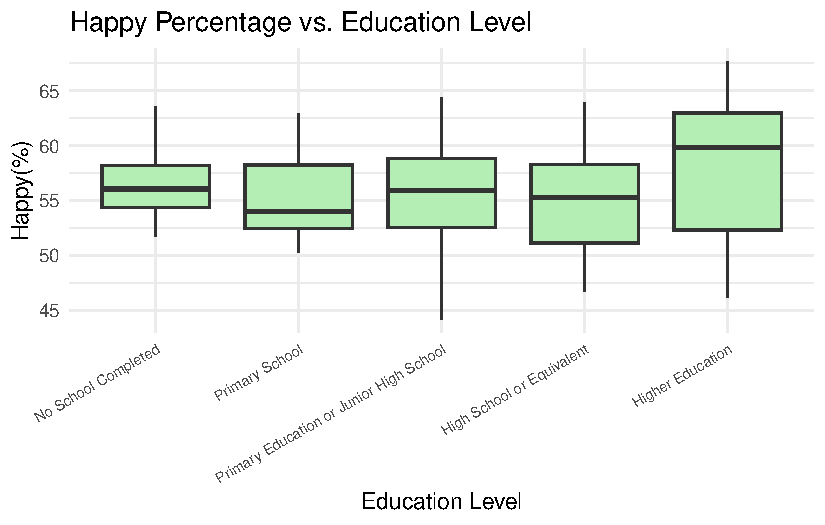
\includegraphics[keepaspectratio]{project_files/figure-pdf/unnamed-chunk-28-1.pdf}}

\begin{Shaded}
\begin{Highlighting}[]
\NormalTok{model2 }\OtherTok{\textless{}{-}} \FunctionTok{lm}\NormalTok{(Percentage }\SpecialCharTok{\textasciitilde{}}\NormalTok{ Education\_Level }\SpecialCharTok{+}\NormalTok{ Year, }\AttributeTok{data =}\NormalTok{ happy\_df\_byeducation)}
\FunctionTok{summary}\NormalTok{(model2)}
\end{Highlighting}
\end{Shaded}

\begin{verbatim}

Call:
lm(formula = Percentage ~ Education_Level + Year, data = happy_df_byeducation)

Residuals:
    Min      1Q  Median      3Q     Max 
-9.4845 -2.4151  0.4029  2.6386  7.8886 

Coefficients:
                                                        Estimate Std. Error
(Intercept)                                            1496.0883   203.9767
Education_LevelPrimary School                            -1.2328     1.4753
Education_LevelPrimary Education or Junior High School   -1.5648     1.4753
Education_LevelHigh School or Equivalent                 -1.3533     1.4753
Education_LevelHigher Education                           1.2962     1.4753
Year                                                     -0.7142     0.1012
                                                       t value Pr(>|t|)    
(Intercept)                                              7.335 2.33e-10 ***
Education_LevelPrimary School                           -0.836    0.406    
Education_LevelPrimary Education or Junior High School  -1.061    0.292    
Education_LevelHigh School or Equivalent                -0.917    0.362    
Education_LevelHigher Education                          0.879    0.382    
Year                                                    -7.057 7.70e-10 ***
---
Signif. codes:  0 '***' 0.001 '**' 0.01 '*' 0.05 '.' 0.1 ' ' 1

Residual standard error: 4.173 on 74 degrees of freedom
Multiple R-squared:  0.4271,    Adjusted R-squared:  0.3884 
F-statistic: 11.04 on 5 and 74 DF,  p-value: 5.843e-08
\end{verbatim}

\begin{Shaded}
\begin{Highlighting}[]
\NormalTok{model3 }\OtherTok{\textless{}{-}} \FunctionTok{lm}\NormalTok{(Percentage }\SpecialCharTok{\textasciitilde{}}\NormalTok{ Education\_Level }\SpecialCharTok{*}\NormalTok{ Year, }\AttributeTok{data =}\NormalTok{ happy\_df\_byeducation)}
\FunctionTok{summary}\NormalTok{(model3)}
\end{Highlighting}
\end{Shaded}

\begin{verbatim}

Call:
lm(formula = Percentage ~ Education_Level * Year, data = happy_df_byeducation)

Residuals:
    Min      1Q  Median      3Q     Max 
-6.9436 -2.1574  0.0044  2.6583  7.7300 

Coefficients:
                                                              Estimate
(Intercept)                                                  234.57621
Education_LevelPrimary School                                620.91983
Education_LevelPrimary Education or Junior High School      1602.28219
Education_LevelHigh School or Equivalent                    1498.40007
Education_LevelHigher Education                             2583.10352
Year                                                          -0.08828
Education_LevelPrimary School:Year                            -0.30868
Education_LevelPrimary Education or Junior High School:Year   -0.79576
Education_LevelHigh School or Equivalent:Year                 -0.74411
Education_LevelHigher Education:Year                          -1.28098
                                                            Std. Error t value
(Intercept)                                                  404.91157   0.579
Education_LevelPrimary School                                572.63143   1.084
Education_LevelPrimary Education or Junior High School       572.63143   2.798
Education_LevelHigh School or Equivalent                     572.63143   2.617
Education_LevelHigher Education                              572.63143   4.511
Year                                                           0.20090  -0.439
Education_LevelPrimary School:Year                             0.28411  -1.086
Education_LevelPrimary Education or Junior High School:Year    0.28411  -2.801
Education_LevelHigh School or Equivalent:Year                  0.28411  -2.619
Education_LevelHigher Education:Year                           0.28411  -4.509
                                                            Pr(>|t|)    
(Intercept)                                                  0.56423    
Education_LevelPrimary School                                0.28194    
Education_LevelPrimary Education or Junior High School       0.00663 ** 
Education_LevelHigh School or Equivalent                     0.01087 *  
Education_LevelHigher Education                             2.53e-05 ***
Year                                                         0.66170    
Education_LevelPrimary School:Year                           0.28099    
Education_LevelPrimary Education or Junior High School:Year  0.00658 ** 
Education_LevelHigh School or Equivalent:Year                0.01080 *  
Education_LevelHigher Education:Year                        2.56e-05 ***
---
Signif. codes:  0 '***' 0.001 '**' 0.01 '*' 0.05 '.' 0.1 ' ' 1

Residual standard error: 3.704 on 70 degrees of freedom
Multiple R-squared:  0.5729,    Adjusted R-squared:  0.518 
F-statistic: 10.43 on 9 and 70 DF,  p-value: 4.852e-10
\end{verbatim}

\begin{Shaded}
\begin{Highlighting}[]
\FunctionTok{AIC}\NormalTok{(model1, model2, model3)}
\end{Highlighting}
\end{Shaded}

\begin{verbatim}
       df      AIC
model1  6 502.5322
model2  7 463.3631
model3 11 447.8703
\end{verbatim}

\begin{Shaded}
\begin{Highlighting}[]
\FunctionTok{ggplot}\NormalTok{(happy\_df\_byeducation, }\FunctionTok{aes}\NormalTok{(}\AttributeTok{sample =} \FunctionTok{resid}\NormalTok{(model3))) }\SpecialCharTok{+}
  \FunctionTok{stat\_qq}\NormalTok{() }\SpecialCharTok{+}
  \FunctionTok{stat\_qq\_line}\NormalTok{(}\AttributeTok{color =} \StringTok{"darkgreen"}\NormalTok{) }\SpecialCharTok{+}
  \FunctionTok{labs}\NormalTok{(}\AttributeTok{title =} \StringTok{"Normal Q{-}Q Plot"}\NormalTok{) }\SpecialCharTok{+}
  \FunctionTok{theme\_clean}\NormalTok{()}
\end{Highlighting}
\end{Shaded}

\pandocbounded{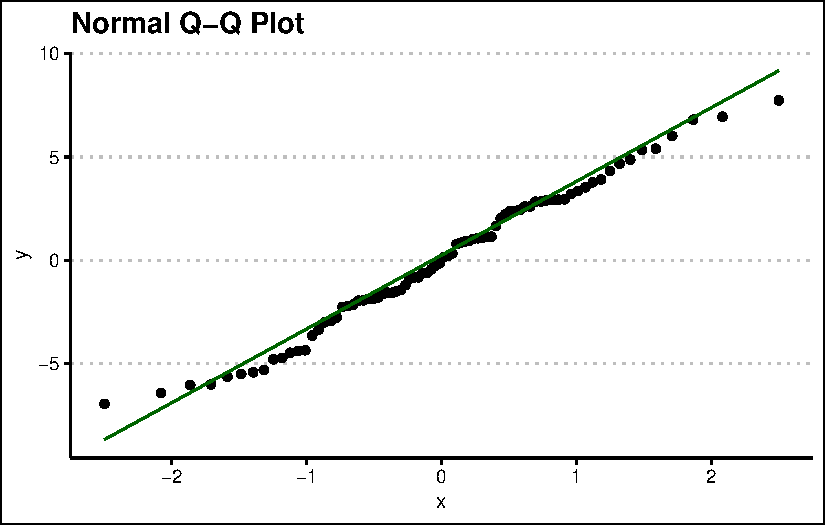
\includegraphics[keepaspectratio]{project_files/figure-pdf/unnamed-chunk-28-2.pdf}}

\begin{Shaded}
\begin{Highlighting}[]
\NormalTok{residuals }\OtherTok{\textless{}{-}} \FunctionTok{resid}\NormalTok{(model3)}

\NormalTok{ad\_test\_results }\OtherTok{\textless{}{-}} \FunctionTok{ad.test}\NormalTok{(residuals)}
\FunctionTok{print}\NormalTok{(ad\_test\_results)}
\end{Highlighting}
\end{Shaded}

\begin{verbatim}

    Anderson-Darling normality test

data:  residuals
A = 0.31572, p-value = 0.5353
\end{verbatim}

\begin{Shaded}
\begin{Highlighting}[]
\NormalTok{edu\_predict}\OtherTok{\textless{}{-}}\FunctionTok{data.frame}\NormalTok{(}\AttributeTok{Education\_Level =} \FunctionTok{factor}\NormalTok{(}
    \FunctionTok{c}\NormalTok{(}\StringTok{"No School Completed"}\NormalTok{,}
      \StringTok{"Primary School"}\NormalTok{,}
      \StringTok{"Primary Education or Junior High School"}\NormalTok{,}
      \StringTok{"High School or Equivalent"}\NormalTok{,}
      \StringTok{"Higher Education"}\NormalTok{),}
    \AttributeTok{levels =} \FunctionTok{levels}\NormalTok{(happy\_df\_byeducation}\SpecialCharTok{$}\NormalTok{Education\_Level)}
\NormalTok{  ),}\AttributeTok{Year=}\FunctionTok{rep}\NormalTok{(}\DecValTok{2024}\SpecialCharTok{:}\DecValTok{2028}\NormalTok{,}\AttributeTok{each=}\DecValTok{5}\NormalTok{)}
\NormalTok{)}
\NormalTok{Prediction}\OtherTok{\textless{}{-}}\FunctionTok{data.frame}\NormalTok{(}\AttributeTok{Prediction=}\FunctionTok{predict}\NormalTok{(model3, }\AttributeTok{newdata =}\NormalTok{ edu\_predict))}
\NormalTok{edu\_predict}\OtherTok{\textless{}{-}}\FunctionTok{bind\_cols}\NormalTok{(edu\_predict,Prediction)}
\FunctionTok{kbl}\NormalTok{(edu\_predict) }\SpecialCharTok{|\textgreater{}} \FunctionTok{kable\_styling}\NormalTok{(}\AttributeTok{full\_width =} \DecValTok{5}\NormalTok{)}
\end{Highlighting}
\end{Shaded}

\begin{tabu} to \linewidth {>{\raggedright}X>{\raggedleft}X>{\raggedleft}X}
\hline
Education\_Level & Year & Prediction\\
\hline
No School Completed & 2024 & 55.89188\\
\hline
Primary School & 2024 & 52.03531\\
\hline
Primary Education or Junior High School & 2024 & 47.56311\\
\hline
High School or Equivalent & 2024 & 48.21365\\
\hline
Higher Education & 2024 & 46.29979\\
\hline
No School Completed & 2025 & 55.80360\\
\hline
Primary School & 2025 & 51.63834\\
\hline
Primary Education or Junior High School & 2025 & 46.67907\\
\hline
High School or Equivalent & 2025 & 47.38126\\
\hline
Higher Education & 2025 & 44.93053\\
\hline
No School Completed & 2026 & 55.71532\\
\hline
Primary School & 2026 & 51.24137\\
\hline
Primary Education or Junior High School & 2026 & 45.79503\\
\hline
High School or Equivalent & 2026 & 46.54887\\
\hline
Higher Education & 2026 & 43.56127\\
\hline
No School Completed & 2027 & 55.62704\\
\hline
Primary School & 2027 & 50.84441\\
\hline
Primary Education or Junior High School & 2027 & 44.91099\\
\hline
High School or Equivalent & 2027 & 45.71647\\
\hline
Higher Education & 2027 & 42.19201\\
\hline
No School Completed & 2028 & 55.53875\\
\hline
Primary School & 2028 & 50.44744\\
\hline
Primary Education or Junior High School & 2028 & 44.02695\\
\hline
High School or Equivalent & 2028 & 44.88408\\
\hline
Higher Education & 2028 & 40.82275\\
\hline
\end{tabu}

\begin{Shaded}
\begin{Highlighting}[]
\FunctionTok{ggplot}\NormalTok{(edu\_predict, }\FunctionTok{aes}\NormalTok{(}\AttributeTok{x =}\NormalTok{ Year, }\AttributeTok{y =}\NormalTok{ Prediction, }\AttributeTok{color =}\NormalTok{ Education\_Level)) }\SpecialCharTok{+}
  \FunctionTok{geom\_line}\NormalTok{() }\SpecialCharTok{+}
  \FunctionTok{geom\_point}\NormalTok{()}\SpecialCharTok{+}
  \FunctionTok{scale\_x\_continuous}\NormalTok{(}\AttributeTok{breaks =} \FunctionTok{seq}\NormalTok{(}\FunctionTok{min}\NormalTok{(edu\_predict}\SpecialCharTok{$}\NormalTok{Year), }\FunctionTok{max}\NormalTok{(edu\_predict}\SpecialCharTok{$}\NormalTok{Year), }\AttributeTok{by =} \DecValTok{1}\NormalTok{))}\SpecialCharTok{+}
  \FunctionTok{labs}\NormalTok{(}\AttributeTok{title =} \StringTok{"Happiness Trend by Education Level Over Years"}\NormalTok{)}\SpecialCharTok{+}
  \FunctionTok{theme\_minimal}\NormalTok{()}
\end{Highlighting}
\end{Shaded}

\pandocbounded{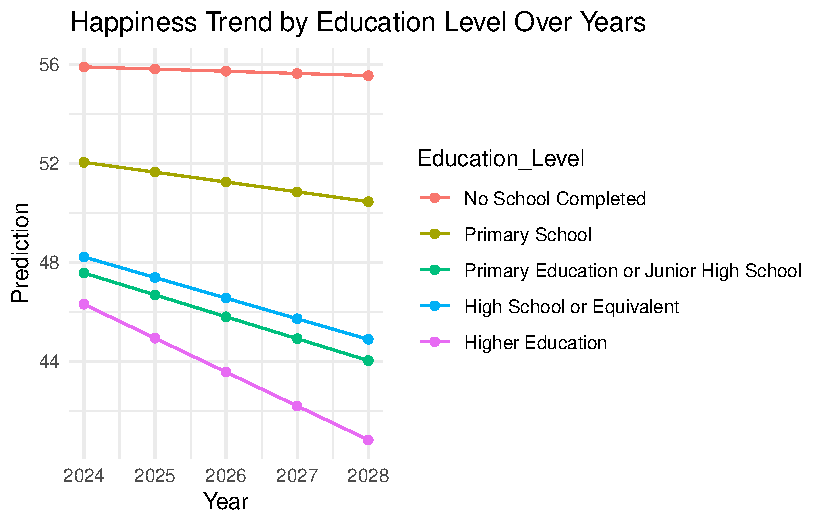
\includegraphics[keepaspectratio]{project_files/figure-pdf/unnamed-chunk-28-3.pdf}}

\textbf{Gender-Based Happiness Level Prediction Model;}

The prediction model for happiness percentages based on gender can be
established in three different ways.

\begin{itemize}
\item
  {\textbf{Model 1}} assumes that the happiness rate is only affected by
  {\textbf{gender}}.
\item
  {\textbf{Model 2}} includes the {\textbf{effect of time}} in the
  prediction model.
\item
  {\textbf{Model 3}} adds the {\textbf{interaction}} between gender and
  time to the prediction model.
\end{itemize}

Based on the results, when the AIC (Akaike Information Criterion)
{[}4{]} values of the models are compared, it is observed that the model
that best explains the data is {\textbf{Model 2, which has the lowest
AIC value}}. Therefore, it can be concluded that the effect of the year
should be included in the constructed prediction model.

Thus, in the prediction model for happiness percentage, the significant
variables, {\textbf{``GenderFemale''}} (which takes a value of 0 for
Male and 1 for Female) and {\textbf{``Year''}}, should be
{\textbf{included}}. Since the ``Gender'' variable is categorical, a
reference category is selected when constructing the model, which is
typically the first level. In this case, the reference category is the
``Male'' category. The ``Intercept''(β₀) value in the model output
represents the average happiness percentage for males, while the
``GenderFemale'' coefficient indicates the difference in the average
happiness percentage between females and males.

According to the model created, the percentages of happiness by gender
between 2024 and 2028 are estimated as follows and shown on the
graph.Parallel to previous findings, it is predicted that happiness
rates will decrease for both genders.

The adequacy of the model was validated by analyzing whether the
residuals conform to a normal distribution with Q-Q Plot and
Anderson-Darling Normality Test.

\begin{Shaded}
\begin{Highlighting}[]
\NormalTok{happy\_df\_bygender  }\OtherTok{\textless{}{-}}\NormalTok{ bygender}\SpecialCharTok{|\textgreater{}}
  \FunctionTok{pivot\_longer}\NormalTok{(}\AttributeTok{cols =} \FunctionTok{c}\NormalTok{(}\StringTok{"Male"}\NormalTok{, }\StringTok{"Female"}\NormalTok{), }
               \AttributeTok{names\_to =} \StringTok{"Gender"}\NormalTok{, }
               \AttributeTok{values\_to =} \StringTok{"Percentage"}\NormalTok{)}\SpecialCharTok{|\textgreater{}}
  \FunctionTok{filter}\NormalTok{(Happiness\_Level }\SpecialCharTok{==} \StringTok{"Happy"}\NormalTok{)}\SpecialCharTok{|\textgreater{}}
\FunctionTok{mutate}\NormalTok{(}\AttributeTok{Gender =} \FunctionTok{factor}\NormalTok{(Gender,}\AttributeTok{levels =} \FunctionTok{c}\NormalTok{(}\StringTok{"Male"}\NormalTok{,}\StringTok{"Female"}\NormalTok{)}
\NormalTok{))}

\NormalTok{model1 }\OtherTok{\textless{}{-}} \FunctionTok{lm}\NormalTok{(Percentage }\SpecialCharTok{\textasciitilde{}}\NormalTok{ Gender, }\AttributeTok{data =}\NormalTok{ happy\_df\_bygender)}
\FunctionTok{summary}\NormalTok{(model1)}
\end{Highlighting}
\end{Shaded}

\begin{verbatim}

Call:
lm(formula = Percentage ~ Gender, data = happy_df_bygender)

Residuals:
    Min      1Q  Median      3Q     Max 
-8.9562 -2.9828  0.1938  3.6625  7.3438 

Coefficients:
             Estimate Std. Error t value Pr(>|t|)    
(Intercept)    52.256      1.171  44.619  < 2e-16 ***
GenderFemale    6.806      1.656   4.109 0.000283 ***
---
Signif. codes:  0 '***' 0.001 '**' 0.01 '*' 0.05 '.' 0.1 ' ' 1

Residual standard error: 4.685 on 30 degrees of freedom
Multiple R-squared:  0.3602,    Adjusted R-squared:  0.3388 
F-statistic: 16.89 on 1 and 30 DF,  p-value: 0.0002825
\end{verbatim}

\begin{Shaded}
\begin{Highlighting}[]
\FunctionTok{ggplot}\NormalTok{(happy\_df\_bygender, }\FunctionTok{aes}\NormalTok{(}\AttributeTok{x =}\NormalTok{ Gender, }\AttributeTok{y =}\NormalTok{ Percentage)) }\SpecialCharTok{+}
  \FunctionTok{geom\_boxplot}\NormalTok{(}\AttributeTok{fill =} \StringTok{"darkseagreen2"}\NormalTok{) }\SpecialCharTok{+}
  \FunctionTok{labs}\NormalTok{(}\AttributeTok{title =} \StringTok{"Happy Percentage vs. Gender"}\NormalTok{,}
       \AttributeTok{x =} \StringTok{"Gender"}\NormalTok{, }\AttributeTok{y =} \StringTok{"Happy (\%)"}\NormalTok{) }\SpecialCharTok{+}
  \FunctionTok{theme\_minimal}\NormalTok{()}
\end{Highlighting}
\end{Shaded}

\pandocbounded{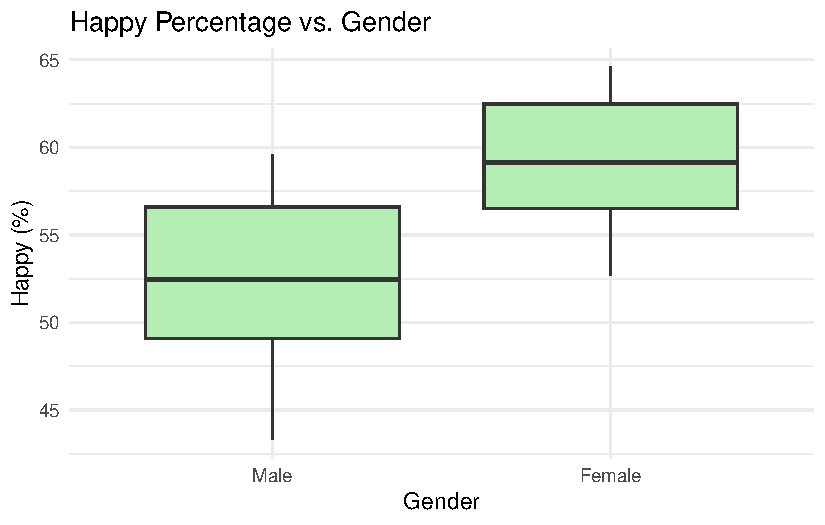
\includegraphics[keepaspectratio]{project_files/figure-pdf/unnamed-chunk-29-1.pdf}}

\begin{Shaded}
\begin{Highlighting}[]
\NormalTok{model2 }\OtherTok{\textless{}{-}} \FunctionTok{lm}\NormalTok{(Percentage }\SpecialCharTok{\textasciitilde{}}\NormalTok{ Gender}\SpecialCharTok{+}\NormalTok{ Year, }\AttributeTok{data =}\NormalTok{ happy\_df\_bygender)}
\FunctionTok{summary}\NormalTok{(model2)}
\end{Highlighting}
\end{Shaded}

\begin{verbatim}

Call:
lm(formula = Percentage ~ Gender + Year, data = happy_df_bygender)

Residuals:
    Min      1Q  Median      3Q     Max 
-6.1588 -2.2183  0.2604  2.3922  6.1670 

Coefficients:
              Estimate Std. Error t value Pr(>|t|)    
(Intercept)  1355.3659   277.6201   4.882 3.52e-05 ***
GenderFemale    6.8063     1.2699   5.360 9.34e-06 ***
Year           -0.6465     0.1377  -4.694 5.94e-05 ***
---
Signif. codes:  0 '***' 0.001 '**' 0.01 '*' 0.05 '.' 0.1 ' ' 1

Residual standard error: 3.592 on 29 degrees of freedom
Multiple R-squared:  0.6364,    Adjusted R-squared:  0.6113 
F-statistic: 25.38 on 2 and 29 DF,  p-value: 4.256e-07
\end{verbatim}

\begin{Shaded}
\begin{Highlighting}[]
\NormalTok{model3 }\OtherTok{\textless{}{-}} \FunctionTok{lm}\NormalTok{(Percentage }\SpecialCharTok{\textasciitilde{}}\NormalTok{ Gender }\SpecialCharTok{*}\NormalTok{ Year, }\AttributeTok{data =}\NormalTok{ happy\_df\_bygender)}
\FunctionTok{summary}\NormalTok{(model3)}
\end{Highlighting}
\end{Shaded}

\begin{verbatim}

Call:
lm(formula = Percentage ~ Gender * Year, data = happy_df_bygender)

Residuals:
    Min      1Q  Median      3Q     Max 
-6.9450 -2.2140  0.1197  2.6519  6.2275 

Coefficients:
                   Estimate Std. Error t value Pr(>|t|)    
(Intercept)       1599.1525   394.2144   4.057 0.000361 ***
GenderFemale      -480.7669   557.5034  -0.862 0.395817    
Year                -0.7675     0.1956  -3.924 0.000515 ***
GenderFemale:Year    0.2419     0.2766   0.875 0.389249    
---
Signif. codes:  0 '***' 0.001 '**' 0.01 '*' 0.05 '.' 0.1 ' ' 1

Residual standard error: 3.607 on 28 degrees of freedom
Multiple R-squared:  0.6461,    Adjusted R-squared:  0.6081 
F-statistic: 17.04 on 3 and 28 DF,  p-value: 1.716e-06
\end{verbatim}

\begin{Shaded}
\begin{Highlighting}[]
\FunctionTok{AIC}\NormalTok{(model1, model2, model3) }
\end{Highlighting}
\end{Shaded}

\begin{verbatim}
       df      AIC
model1  3 193.5824
model2  4 177.4970
model3  5 178.6346
\end{verbatim}

\begin{Shaded}
\begin{Highlighting}[]
\FunctionTok{ggplot}\NormalTok{(happy\_df\_bygender, }\FunctionTok{aes}\NormalTok{(}\AttributeTok{sample =} \FunctionTok{resid}\NormalTok{(model2))) }\SpecialCharTok{+}
  \FunctionTok{stat\_qq}\NormalTok{() }\SpecialCharTok{+}
  \FunctionTok{stat\_qq\_line}\NormalTok{(}\AttributeTok{color =} \StringTok{"darkgreen"}\NormalTok{) }\SpecialCharTok{+}
  \FunctionTok{labs}\NormalTok{(}\AttributeTok{title =} \StringTok{"Normal Q{-}Q Plot"}\NormalTok{) }\SpecialCharTok{+}
  \FunctionTok{theme\_clean}\NormalTok{()}
\end{Highlighting}
\end{Shaded}

\pandocbounded{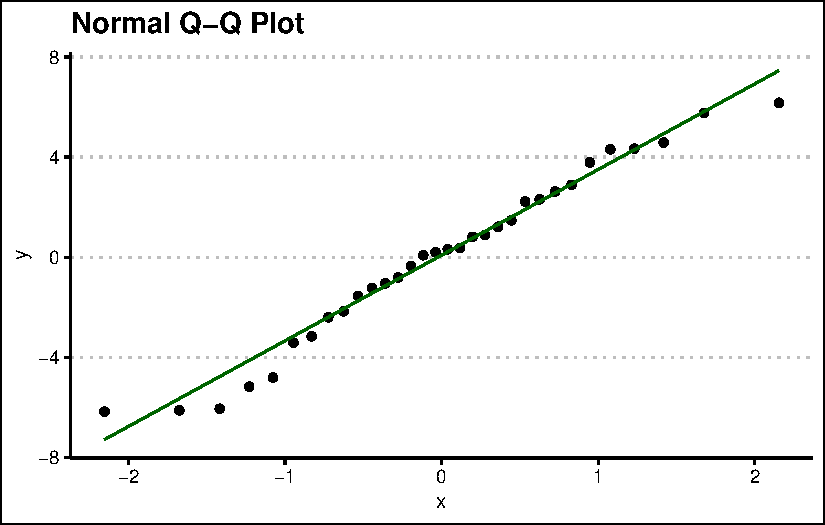
\includegraphics[keepaspectratio]{project_files/figure-pdf/unnamed-chunk-29-2.pdf}}

\begin{Shaded}
\begin{Highlighting}[]
\NormalTok{residuals }\OtherTok{\textless{}{-}} \FunctionTok{resid}\NormalTok{(model2)}

\NormalTok{ad\_test\_results }\OtherTok{\textless{}{-}} \FunctionTok{ad.test}\NormalTok{(residuals)}
\FunctionTok{print}\NormalTok{(ad\_test\_results)}
\end{Highlighting}
\end{Shaded}

\begin{verbatim}

    Anderson-Darling normality test

data:  residuals
A = 0.22885, p-value = 0.793
\end{verbatim}

\begin{Shaded}
\begin{Highlighting}[]
\NormalTok{gender\_predict}\OtherTok{\textless{}{-}}\FunctionTok{data.frame}\NormalTok{(}\AttributeTok{Gender =} \FunctionTok{factor}\NormalTok{(}
    \FunctionTok{c}\NormalTok{(}\StringTok{"Male"}\NormalTok{,}
      \StringTok{"Female"}\NormalTok{),}
    \AttributeTok{levels =} \FunctionTok{levels}\NormalTok{(happy\_df\_bygender}\SpecialCharTok{$}\NormalTok{Gender)}
\NormalTok{  ),}\AttributeTok{Year=}\FunctionTok{rep}\NormalTok{(}\DecValTok{2024}\SpecialCharTok{:}\DecValTok{2028}\NormalTok{,}\AttributeTok{each=}\DecValTok{2}\NormalTok{)}
\NormalTok{)}
\NormalTok{Prediction}\OtherTok{\textless{}{-}}\FunctionTok{data.frame}\NormalTok{(}\AttributeTok{Prediction=}\FunctionTok{predict}\NormalTok{(model2, }\AttributeTok{newdata =}\NormalTok{ gender\_predict))}
\NormalTok{gender\_predict}\OtherTok{\textless{}{-}}\FunctionTok{bind\_cols}\NormalTok{(gender\_predict,Prediction)}
\FunctionTok{kbl}\NormalTok{(gender\_predict) }\SpecialCharTok{|\textgreater{}} \FunctionTok{kable\_styling}\NormalTok{(}\AttributeTok{full\_width =} \DecValTok{5}\NormalTok{)}
\end{Highlighting}
\end{Shaded}

\begin{tabu} to \linewidth {>{\raggedright}X>{\raggedleft}X>{\raggedleft}X}
\hline
Gender & Year & Prediction\\
\hline
Male & 2024 & 46.76062\\
\hline
Female & 2024 & 53.56688\\
\hline
Male & 2025 & 46.11408\\
\hline
Female & 2025 & 52.92033\\
\hline
Male & 2026 & 45.46754\\
\hline
Female & 2026 & 52.27379\\
\hline
Male & 2027 & 44.82099\\
\hline
Female & 2027 & 51.62724\\
\hline
Male & 2028 & 44.17445\\
\hline
Female & 2028 & 50.98070\\
\hline
\end{tabu}

\begin{Shaded}
\begin{Highlighting}[]
\FunctionTok{ggplot}\NormalTok{(gender\_predict, }\FunctionTok{aes}\NormalTok{(}\AttributeTok{x =}\NormalTok{ Year, }\AttributeTok{y =}\NormalTok{ Prediction, }\AttributeTok{color =}\NormalTok{ Gender)) }\SpecialCharTok{+}
  \FunctionTok{geom\_line}\NormalTok{() }\SpecialCharTok{+}
  \FunctionTok{geom\_point}\NormalTok{()}\SpecialCharTok{+}
  \FunctionTok{scale\_x\_continuous}\NormalTok{(}\AttributeTok{breaks =} \FunctionTok{seq}\NormalTok{(}\FunctionTok{min}\NormalTok{(gender\_predict}\SpecialCharTok{$}\NormalTok{Year), }\FunctionTok{max}\NormalTok{(gender\_predict}\SpecialCharTok{$}\NormalTok{Year), }\AttributeTok{by =} \DecValTok{1}\NormalTok{))}\SpecialCharTok{+}
  \FunctionTok{scale\_color\_manual}\NormalTok{(}\AttributeTok{values =} \FunctionTok{c}\NormalTok{(}\StringTok{"Female"} \OtherTok{=} \StringTok{"salmon"}\NormalTok{, }\StringTok{"Male"} \OtherTok{=} \StringTok{"darkslategray3"}\NormalTok{))}\SpecialCharTok{+}
  \FunctionTok{labs}\NormalTok{(}\AttributeTok{title =} \StringTok{"Happiness Trend by Gender Over Years"}\NormalTok{)}\SpecialCharTok{+}
  \FunctionTok{theme\_minimal}\NormalTok{()}
\end{Highlighting}
\end{Shaded}

\pandocbounded{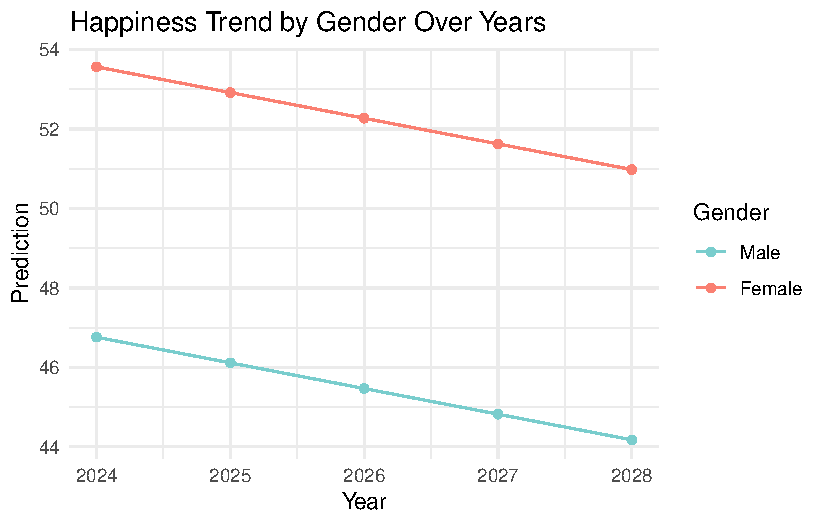
\includegraphics[keepaspectratio]{project_files/figure-pdf/unnamed-chunk-29-3.pdf}}

\section[4. Results and Key Takeaways \hfill
]{\texorpdfstring{4. Results and Key Takeaways
\protect
\includegraphics[width=0.3in,height=\textheight,keepaspectratio]{assets/images/results.png}\hfill
}{4. Results and Key Takeaways }}\label{results-and-key-takeaways}

In this study, three different datasets were analyzed to investigate the
direction and magnitude of the effects of factors such as gender and
educational attainment on individuals' self-reported happiness. These
datasets provide information on the total number of individuals by
education level across different provinces of Turkey over the years, as
well as gender distribution, and the levels of happiness individuals
reported over time based on their education level and gender. The study
was conducted using this information.

During the analysis phase, the first step involved examining the
structure and trends of the variables to gain more detailed insight into
the data. These initial observations were enriched further by exploring
how the variables behaved over time. Finally, the effects of the
variables on happiness percentages were discussed, and regression models
based on gender and education level were developed to predict
individuals' likelihood of reporting happiness.

The key findings from the analysis are summarized below:

\begin{itemize}
\item
  Over time, {\textbf{Istanbul}}, {\textbf{Ankara}}, and
  {\textbf{Izmir}} were identified as the provinces with the {[}greatest
  increase in individuals who either had no formal education or had
  completed university and higher education. While the increase in
  higher education levels in Istanbul and Izmir was more stable,
  {\textbf{Ankara saw a rapid rise}}, especially after 2020. On a
  national scale, the majority of individuals {\textbf{without formal
  education or with only primary education are women}}. In contrast, the
  opposite is true for {\textbf{higher education levels, where men are
  in the majority}}.
\item
  Individuals who identified themselves as {\textbf{happy}} were mostly
  those with {\textbf{higher education}}, whereas those who identified
  as {\textbf{unhappy}} were predominantly individuals {\textbf{without
  any formal education}}. However, the percentage of individuals
  reporting happiness has decreased across all education levels over
  time. The smallest decrease occurred among those with {\textbf{no
  formal education (−0.0089)}}, while the largest decrease was among
  those with {\textbf{higher education (−1.369)}}. For individuals
  reporting unhappiness, the percentage decreased over time only for
  those {\textbf{without education (−0.065)}}, while it increased across
  all other education levels. The highest increase in unhappiness was
  observed among individuals with {\textbf{higher education (+0.45)}}.
\item
  Individuals who identified themselves as {\textbf{happy were mostly
  women}}, while those who reported being unhappy were mostly men. In
  addition, the {\textbf{difference}} in happiness rates between men and
  women who reported being happy has {\textbf{decreased by an average of
  0.24 points per year}}. On the other hand, the difference between men
  and women who reported being unhappy has {\textbf{increased by
  approximately 0.17}} points annually.
\item
  To estimate happiness percentages, various regression models were
  developed based on gender and education level. Models including both
  main effects and interaction terms for relevant factors were compared.
  The best-fitting model was identified based on the Akaike Information
  Criterion (AIC). In the {\textbf{gender-based model}}, the inclusion
  of the time variable (year) alongside {\textbf{gender improved the
  model}} fit. In the education-level model, main effects for primary
  school, high school, and higher education levels, as well as their
  interactions with time, were included in the model specification.
\end{itemize}

According to these results, it is seen that educational disadvantage,
especially in recent years, affects not only women but also men. The
reasons for this should be considered from different perspectives and
steps should be taken towards a solution. The level of education that
individuals have creates a difference in their perspective and
expectations on life and the level of happiness they define themselves
in this way changes to a great extent. The fact that the percentage of
people who do not receive any education feeling unhappy has increased
over time, even if only slightly, has actually proven the saying that
ignorance is bliss, the meaning of which we examine from a different
perspective. Although women seem happier in general in the country, it
should be approached with skepticism as to whether this reflects the
truth in the living conditions we live in. When approached with this
suspicion, the real truth is that the difference in happiness between
men and women decreases over time, and women feel unhappier day by day.

*Assistance from ChatGPT was utilized at certain parts of this study.

The mini research paper related to this study can be accessed
\href{assets/documents/Paper.pdf}{here}.

\section{References}\label{references}

1.Turkish Statistical Institute (TURKSTAT). ``\emph{Life Satisfaction
Survey, 2023''}. Retrieved from \url{https://data.tuik.gov.tr/}
(accessed May, 2025)

2.Turkish Statistical Institute (TURKSTAT).(2024). ``\emph{Population
Statics Portal, 2024''}. Retrieved from \url{https://nip.tuik.gov.tr/}
(accessed May, 2025)

3.K. Pearson, ``\emph{On the criterion that a given system of deviations
from the probable in the case of a correlated system of variables is
such that it can be reasonably supposed to have arisen from random
sampling,}'' The London, Edinburgh, and Dublin Philosophical Magazine
and Journal of Science, vol.~50, no. 302, pp.~157--175, 1900.

4.H. Akaike, ``\emph{A new look at the statistical model
identification,}'' IEEE Transactions on Automatic Control, vol.~19, no.
6, pp.~716--723, 1974.

5.D. Firth and R. Menezes, ``\emph{Quasi-variances,}'' Biometrika,
vol.~91, no. 1, pp.~65--80, 2004.

6.T. W. Anderson and D. A. Darling, ``\emph{A test of goodness of
fit,}'' Journal of the American Statistical Association, vol.~49, no.
268, pp.~765--769, 1954.




\end{document}
